

The following section proposes a teaching scenario in which the interactive subjects are a teacher and a classroom, where the proposed tool is used to explain eXplainable Artificial Intelligence concepts.

The teacher prepares for an advanced machine learning seminar where they will introduce students to eXplainable AI methods, specifically focusing on local explanation techniques that generate synthetic neighborhoods and extract symbolic decision rules and their explaniability method of choice is $\text{LORE}_{sa}$. 
They recognize that previous approaches to teaching these concepts through the textual rule representations presented significant pedagogical challenges. 
When students examined traditional explanation outputs consisting of nested dictionaries containing premises, consequences, and counterfactual conditions, they struggled to build an intuitive understanding of how these logical structures related to the actual decision-making process. The cognitive load of parsing multiple rule conditions while simultaneously trying to understand their interpretation in feature space created a barrier in learning.

The teacher decides to use the interactive visualization system and the Iris dataset for the demonstration. The Iris dataset offers intuitive semantics that help students focus on understanding explanation mechanisms rather than wrestling with domain complexity.

\subsection{Initial Configuration and Conceptual Foundation}

The teacher navigates to the demonstration interface and begins by selecting the Iris dataset. As they click the dataset card, the system reveals the classifier selection interface, and they explain to students why a Random Forest classifier with default parameters is chosen: Random forests operate as black-box ensembles, making their individual predictions difficult to interpret despite their strong performance. This opacity motivates the need for explanation methods that can reveal the decision logic for specific instances.

On top of that, the interface allows the teacher to showcase the dataset in its entirety by the click of the \texttt{Show Dataset} button. Allowing the students to observe the actual values of the dataset in use, as shown in Figure \ref{fig:showDatasetIris}.

\begin{figure}[h]
    \centering
    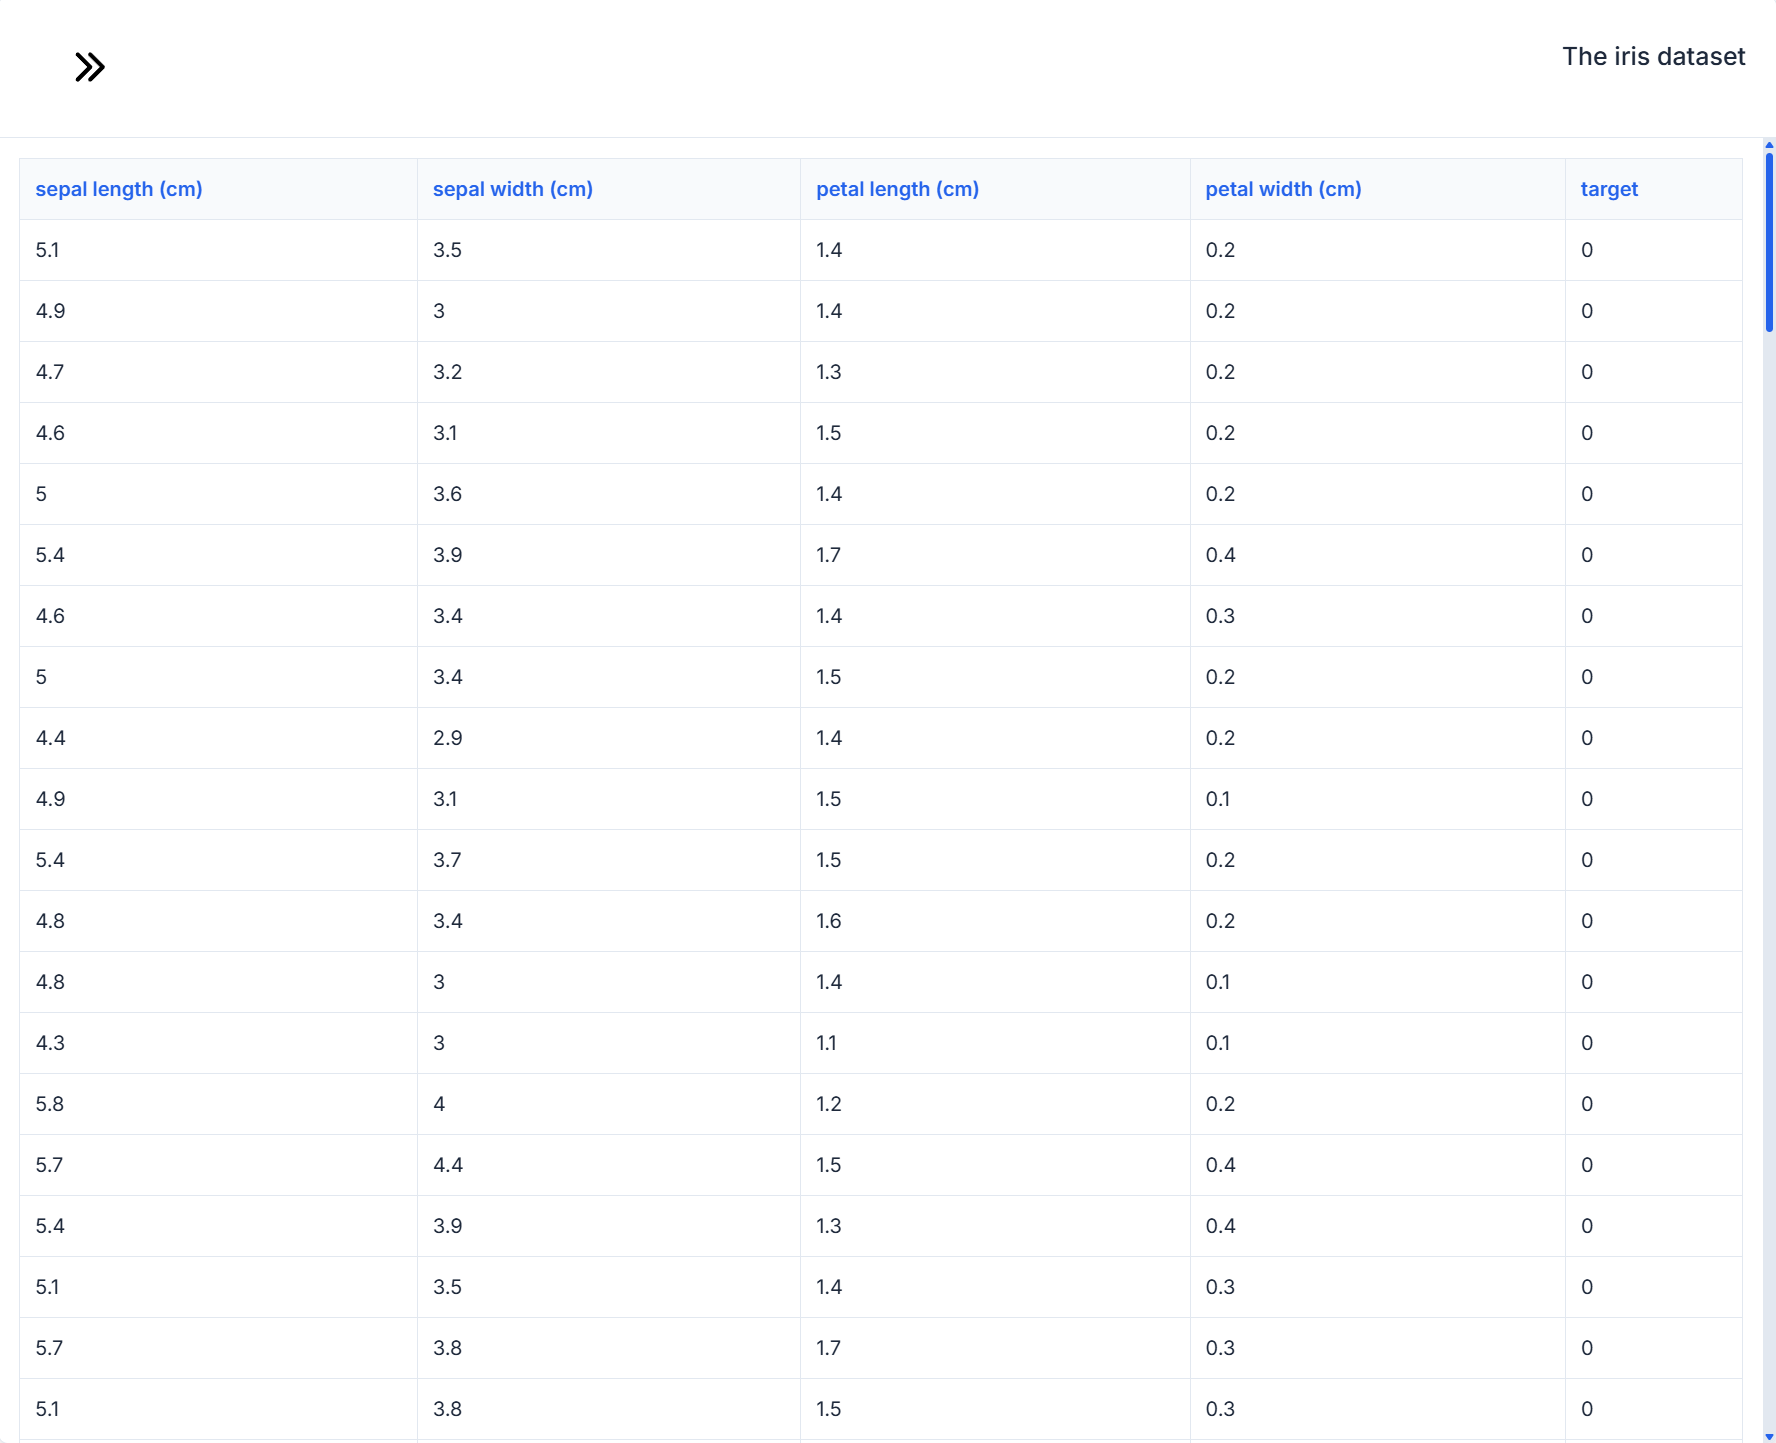
\includegraphics[width=0.7\linewidth]{images/showDatasetIris.png}
    \caption{Iris dataset snippet shown at the click of the \texttt{Show Dataset} button}
    \label{fig:showDatasetIris}
\end{figure}

The interface automatically displays the feature input section, organizing the four Iris features into their numerical group. The teacher observes the median default values populated in each field: sepal length (5.80 cm), sepal width (3.00 cm), petal length (4.35 cm), and petal width (1.30 cm), and uses this moment to introduce a fundamental concept: These median values represent a typical instance from the dataset. When we explain a prediction for this instance, we are learning about how the classifier behaves in a common region of the feature space, not at an extreme edge case.

The teacher scrolls to the Explanation Parameters section and highlights the neighborhood size control, currently set to 500 instances. This parameter determines how many synthetic instances the explanation method generates around our target instance. This parameter is controlling the size of our local investigation, answering the question: How does the classifier behave in this specific neighborhood of feature space? They lower the default value, noting that for the relatively simple Iris dataset, 200 instances provide more than adequate coverage of the local decision space, over the 150 total samples of the dataset.

The teacher leaves the dimensionality reduction parameters at their defaults and enables the original dataset overlay option, explaining that by including the original training data in the visualization, they can observe how the synthetic neighborhood relates to the actual data distribution. This helps in assessing whether the local explanation captures realistic regions of the feature space.

They select the Rule and Counterfactual Rules Centered visualization from the tree layout options, as shown in Figure \ref{fig:teaching_config_complete}, reasoning that its rectangular node structure and guaranteed bottom positioning of the explained instance path provides the clearest initial introduction to decision tree structure. With configuration complete, they click the \texttt{Explain!} button and the system later displays the results of the explanation.

\begin{figure}
    \centering
    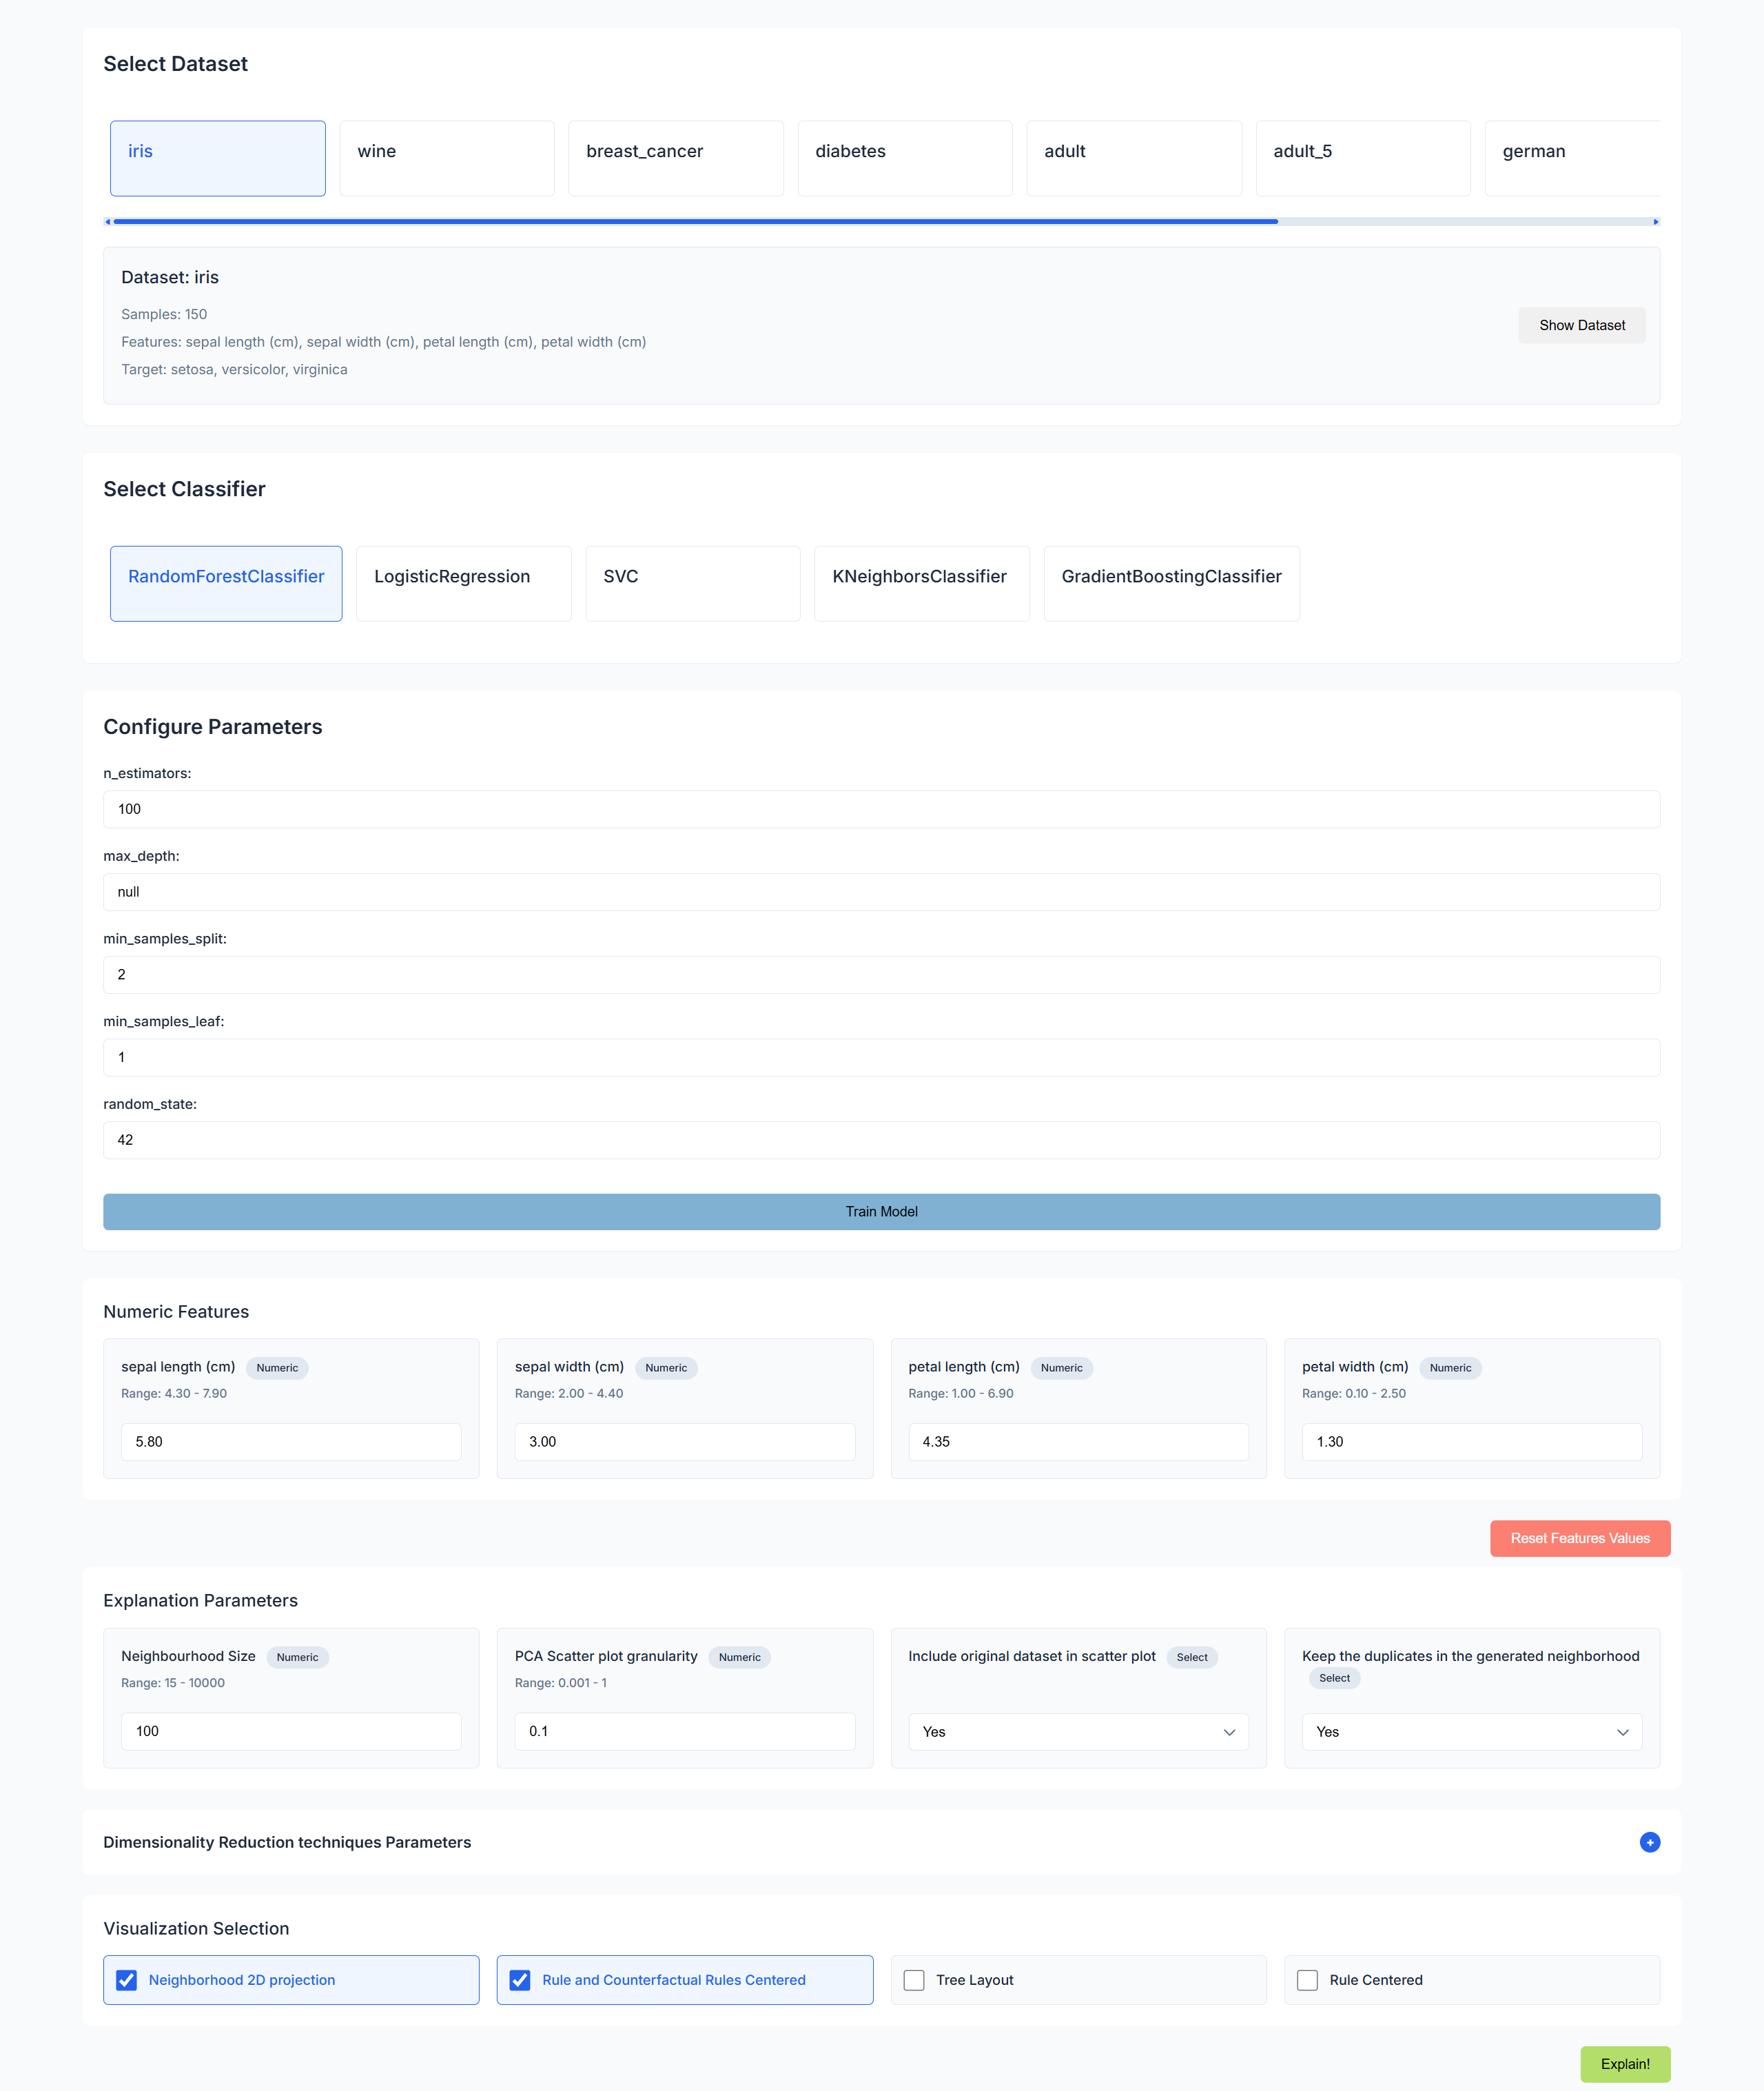
\includegraphics[width=\linewidth]{images/fullConfigTeacher.png}
    \caption{Complete configuration of the system before generating the explanation for the iris dataset's instance.}
    \label{fig:teaching_config_complete}
\end{figure}

\subsection{First Encounter: Understanding Spatial Neighborhoods}

When the visualizations appear, the teacher directs students' attention first to the 2D spatial neighborhood projection, displayed with UMAP dimensionality reduction as shown in Figure \ref{fig:teaching_scatter_initial}. The plot reveals four distinct clusters of points, color-coded in \#FEFEBB (setosa), \#D9E6F5 (versicolor), \#a1dab4 (virginica), and a mixed one with \#D9E6F5 (versicolor), \#a1dab4 (virginica), with the explained instance marked by the star symbol within the versicolor cluster.

The teacher focuses the attention of the students on how the dimensionality reduction has organized the four-dimensional Iris feature space into this two-dimensional projection. The teacher points out that the spatial separation between clusters immediately reveals something important about the classification task: setosa flowers are clearly distinct from the other two species, while versicolor and virginica show some overlap in their decision boundaries.

The teacher hovers over several points in the scatter plot, and students observe the tooltip displaying feature values and class predictions. The teacher highlights how the synthetic instances are concentrated more densely near the explained instance, and notes that this is not a random occurrence. The genetic algorithm that generated these instances specifically optimizes for neighborhood quality, creating some instances, shown in Figures \ref{fig:hoverDecisionBoundaryIrisUmap1} and \ref{fig:hoverDecisionBoundaryIrisUmap2}, near decision boundaries where the classification behavior is most interesting. This observation provides the first opportunity to contrast with the limitations of previous approaches: If we were looking at the traditional textual output, we would see a list of counterfactual samples with their feature values, but we would have no intuitive sense of how these instances are distributed in space. The visualization makes this distribution immediately comprehensible.

\begin{figure}
    \centering
    % Main big image on the left
    \begin{subfigure}[c]{0.65\textwidth}
        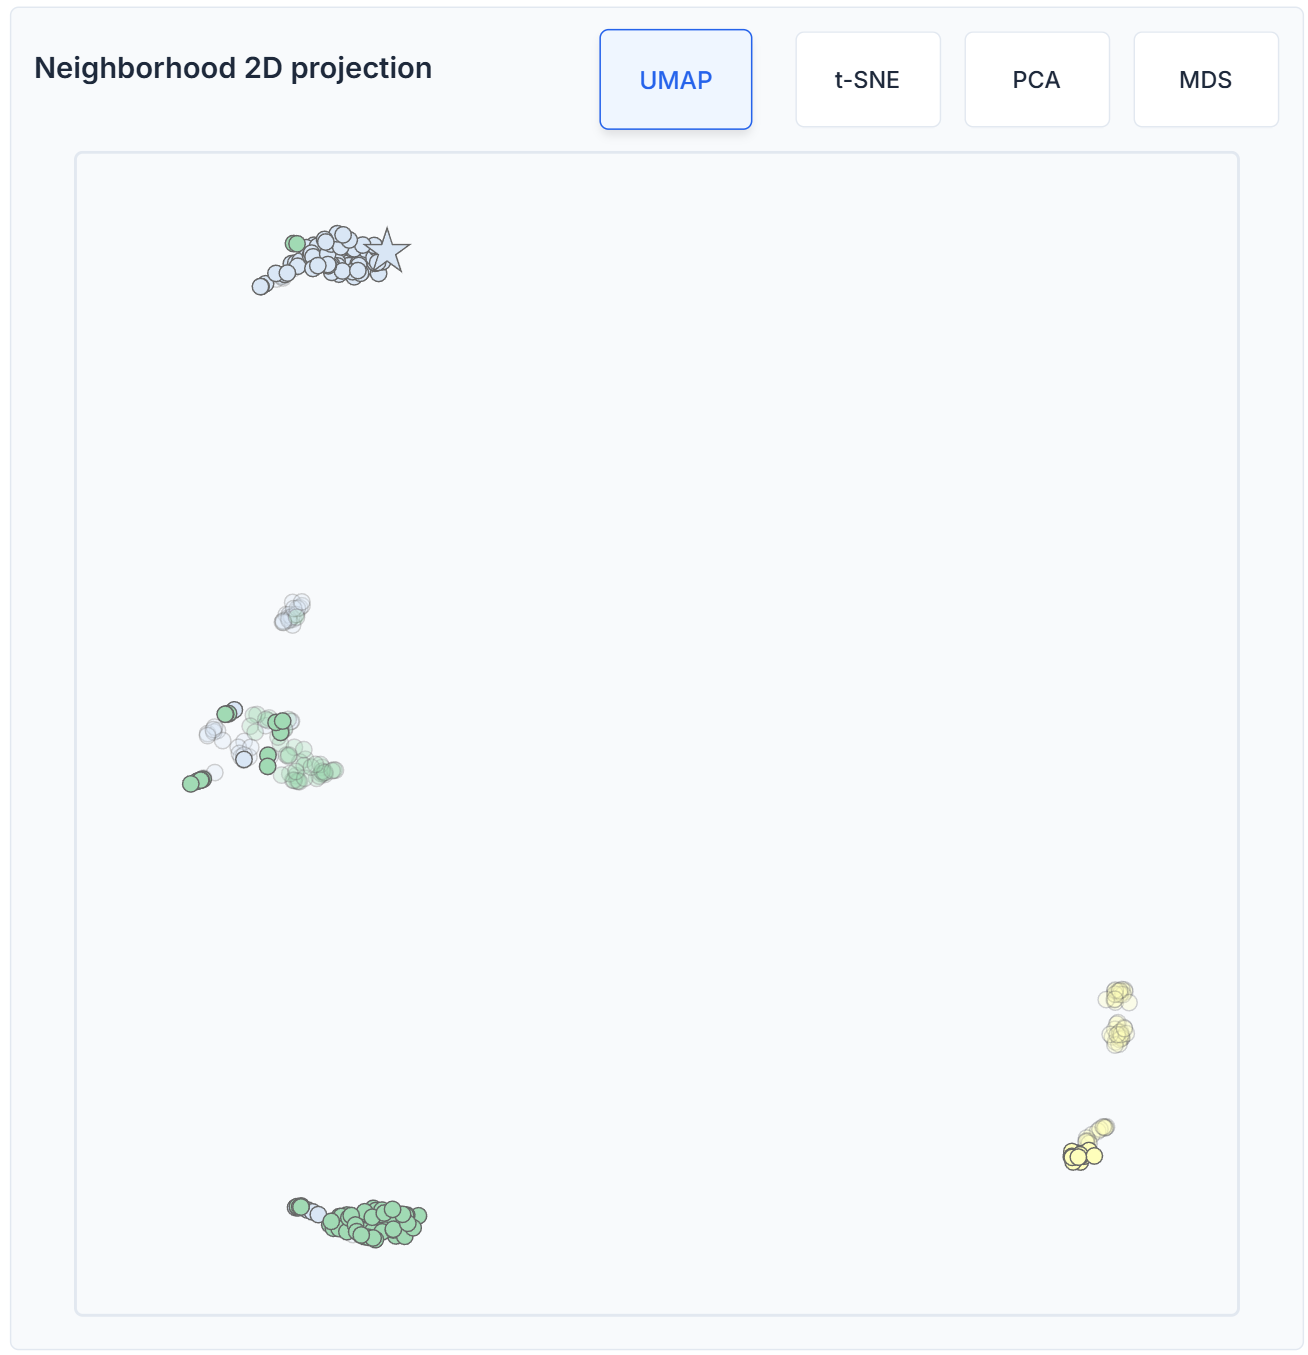
\includegraphics[width=\textwidth]{images/teaching_scatter_initial.png}
        \caption{Neighborhood 2D projection}
        \label{fig:teaching_scatter_initial}
    \end{subfigure}
    \hfill
    % Two stacked images on the right
    \begin{subfigure}[c]{0.33\textwidth}
        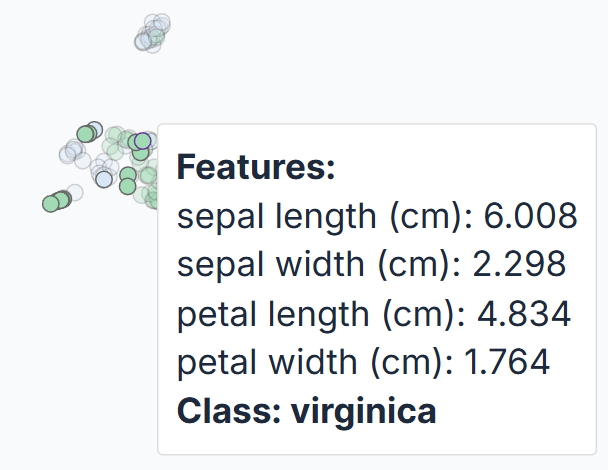
\includegraphics[width=\textwidth]{images/teaching_scatter_initial_virginica_instance.png}
        \caption{Virginica class instance near the decision boundary.}
        \label{fig:hoverDecisionBoundaryIrisUmap1}
        \vfill
        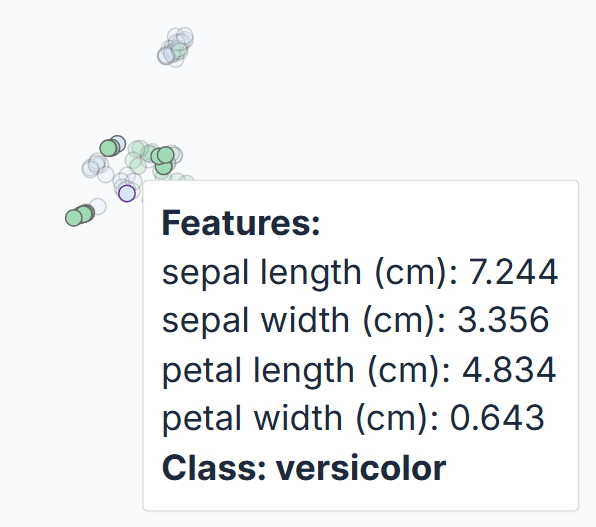
\includegraphics[width=\textwidth]{images/teaching_scatter_initial_versicolor_instance.png}
        \caption{Versicolor class instance near the decision boundary.}
        \label{fig:hoverDecisionBoundaryIrisUmap2}
    \end{subfigure}
    \caption{Initial scatter plot on the Iris dataset using UMAP dimensionality reduction.}
\end{figure}

The teacher clicks the UMAP radio button off and selects t-SNE instead, as shown in Figure \ref{fig:teaching_scatter_tsne}. The projection reorganizes, maintaining the three-cluster structure but with different spatial relationships. 
For teaching purposes, being able to switch between these projections helps understanding that there is no single 'correct' way to visualize high-dimensional data and that each technique offers different insights. 
The teacher later switches to PCA, noting how the linear projection creates a different perspective where the explained instance sits at the boundary between clusters rather than clearly within one. 
The decision boundaries generated by the linear surrogate model are now visible on the Neighborhood 2D projection, and the students have a glimpse of how the decision space is divided by the model, as shown in Figure \ref{fig:teaching_scatter_pca}.

\begin{figure}[ht]
    \centering
    \begin{subfigure}[c]{0.48\textwidth}
        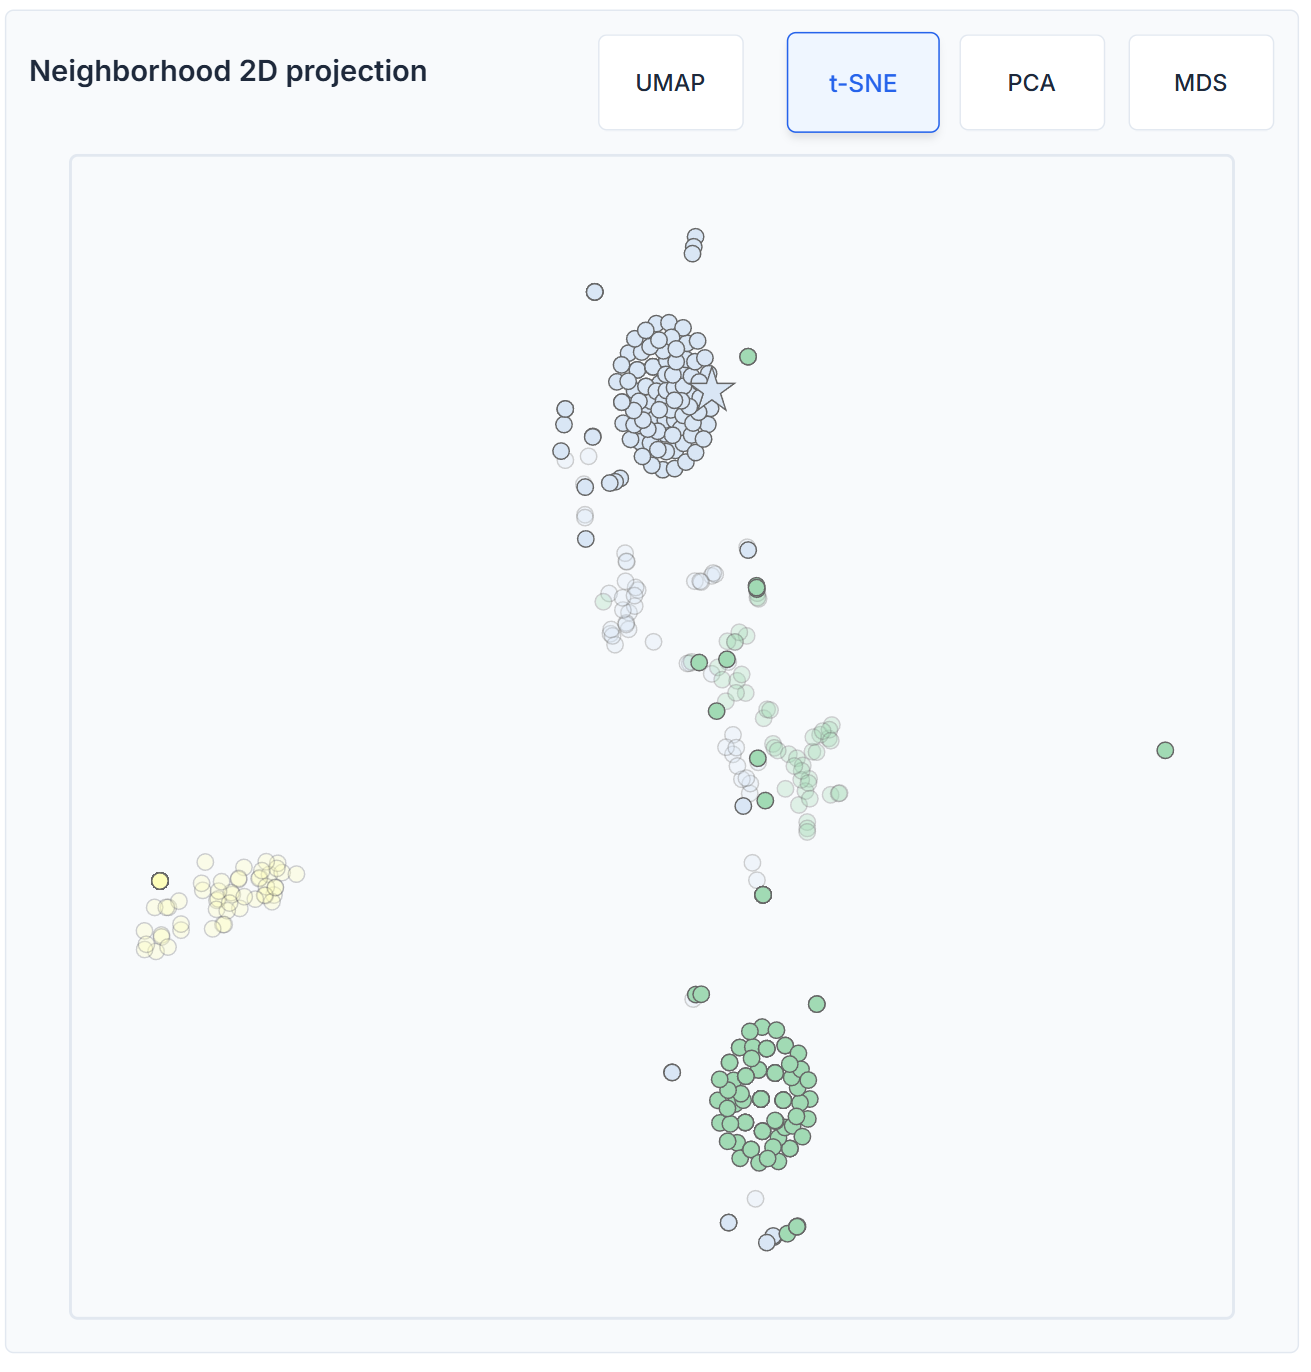
\includegraphics[width=\textwidth]{images/teaching_scatter_tsne.png}
        \caption{t-SNE projection of the generated neighborhood.}
        \label{fig:teaching_scatter_tsne}
    \end{subfigure}
    \hfill
    \begin{subfigure}[c]{0.48\textwidth}
        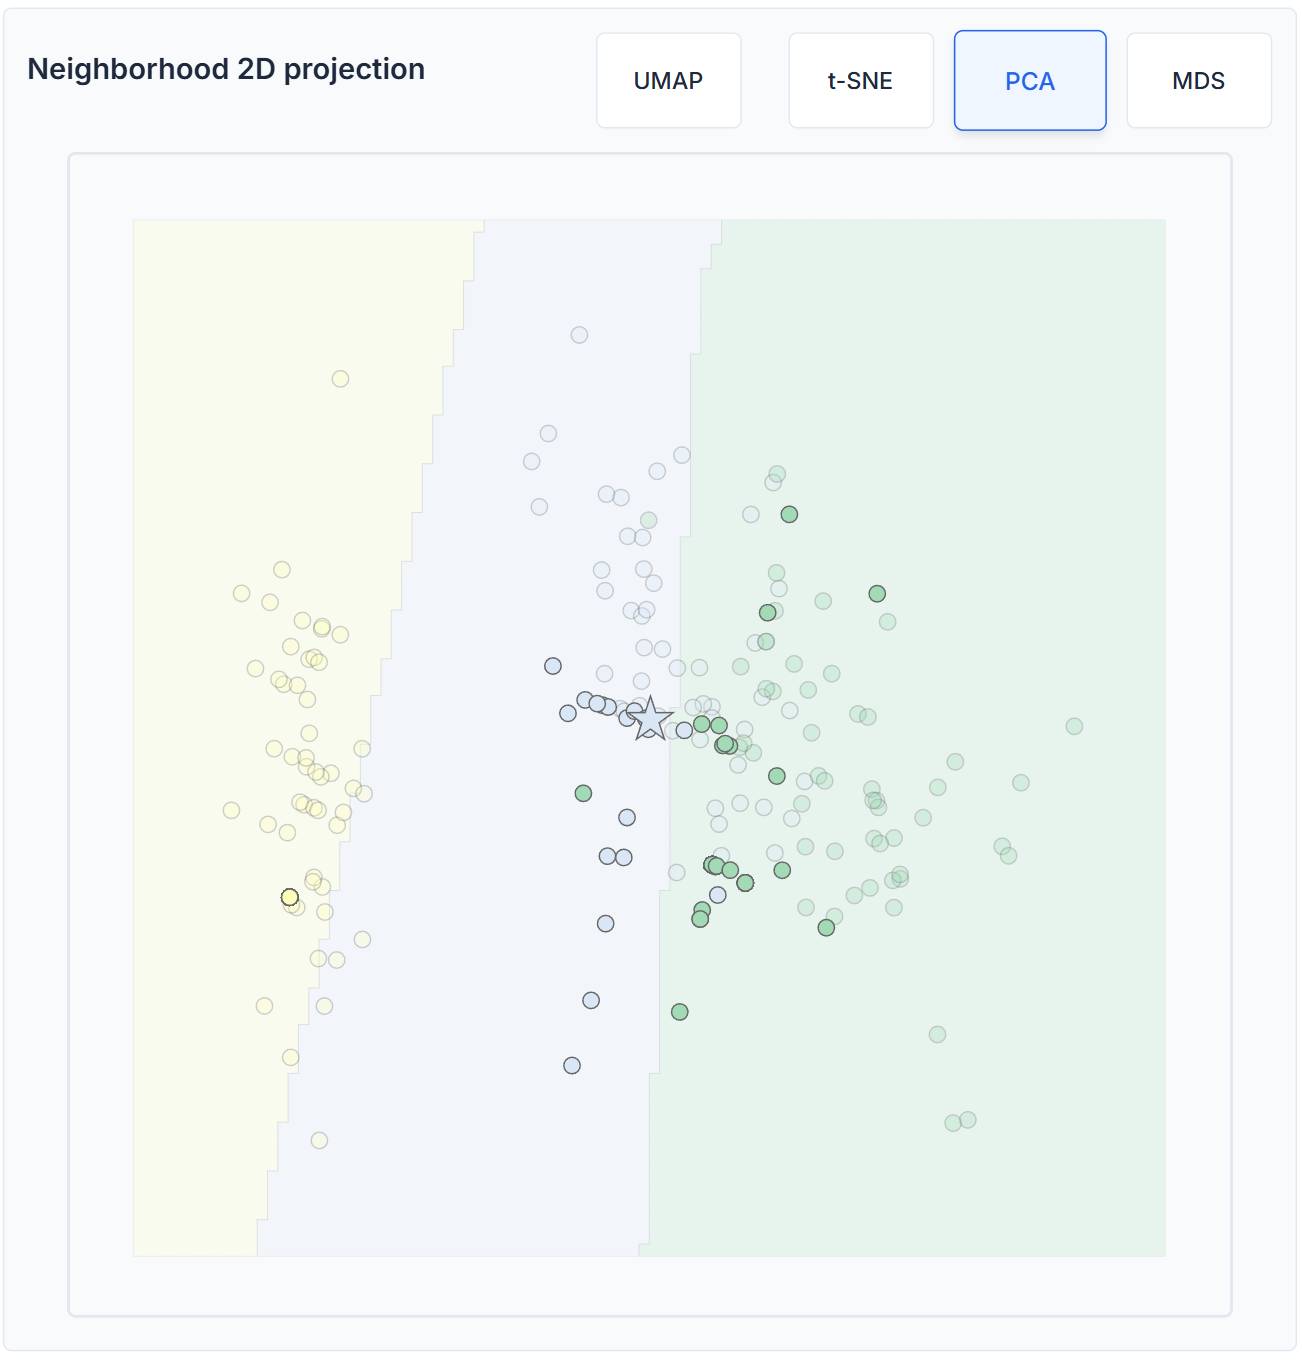
\includegraphics[width=\textwidth]{images/teaching_scatter_pca.png}
        \caption{PCA projection of the generated neighborhood, with decision boundaries displayed.}
        \label{fig:teaching_scatter_pca}
    \end{subfigure}
    \caption{t-SNE and PCA projection of the generated neighborhood.}
\end{figure}


\subsection{Navigating Decision Tree Structure}

Having established spatial intuition about the neighborhood, the teacher shifts focus to the Rule and Counterfactual Rules Centered visualization displayed next to the scatter plot. The tree structure, shown in Figure \ref{fig:teaching_blocks_initial}, presents rectangular nodes arranged in depth-aligned rows, with the explained instance path highlighted at the bottom through enhanced rectangular nodes connected by thick edges.

The shown surrogate model approximates how the Random Forest behaves in the neighborhood they just examined. They trace their cursor along the highlighted path from root to leaf: The instance starts at the root node, where the tree tests whether petal length is less than or equal to 4.4 centimeters. Since our instance has a petal length of 4.35 cm, it takes the true branch.
The teacher hovers over the root node, and students see the tooltip reveal detailed statistics as shown in Figure \ref{fig:teaching_blocks_root_tooltip}: the split condition, impurity measure, sample count, and class distribution. Later the teacher also hovers the leaf node related to the prediction to show the number of samples relative to the predicted class, as shown in Figure \ref{fig:teaching_blocks_prediction_tooltip}.

The teacher continues tracing the path and shows how, at the next level, the tree splits on the petal width feature twice. The chosen instance is lower than the threshold in the first instance, taking the true branch, and later it is higher, taking the false branch. The highlighted path provides the user with the factual rule, otherwise said, the conjunction of conditions that led to the versicolor prediction for this specific instance.

\begin{figure}
    \centering
    % Main big image on the left
    \begin{subfigure}[c]{0.65\textwidth}
        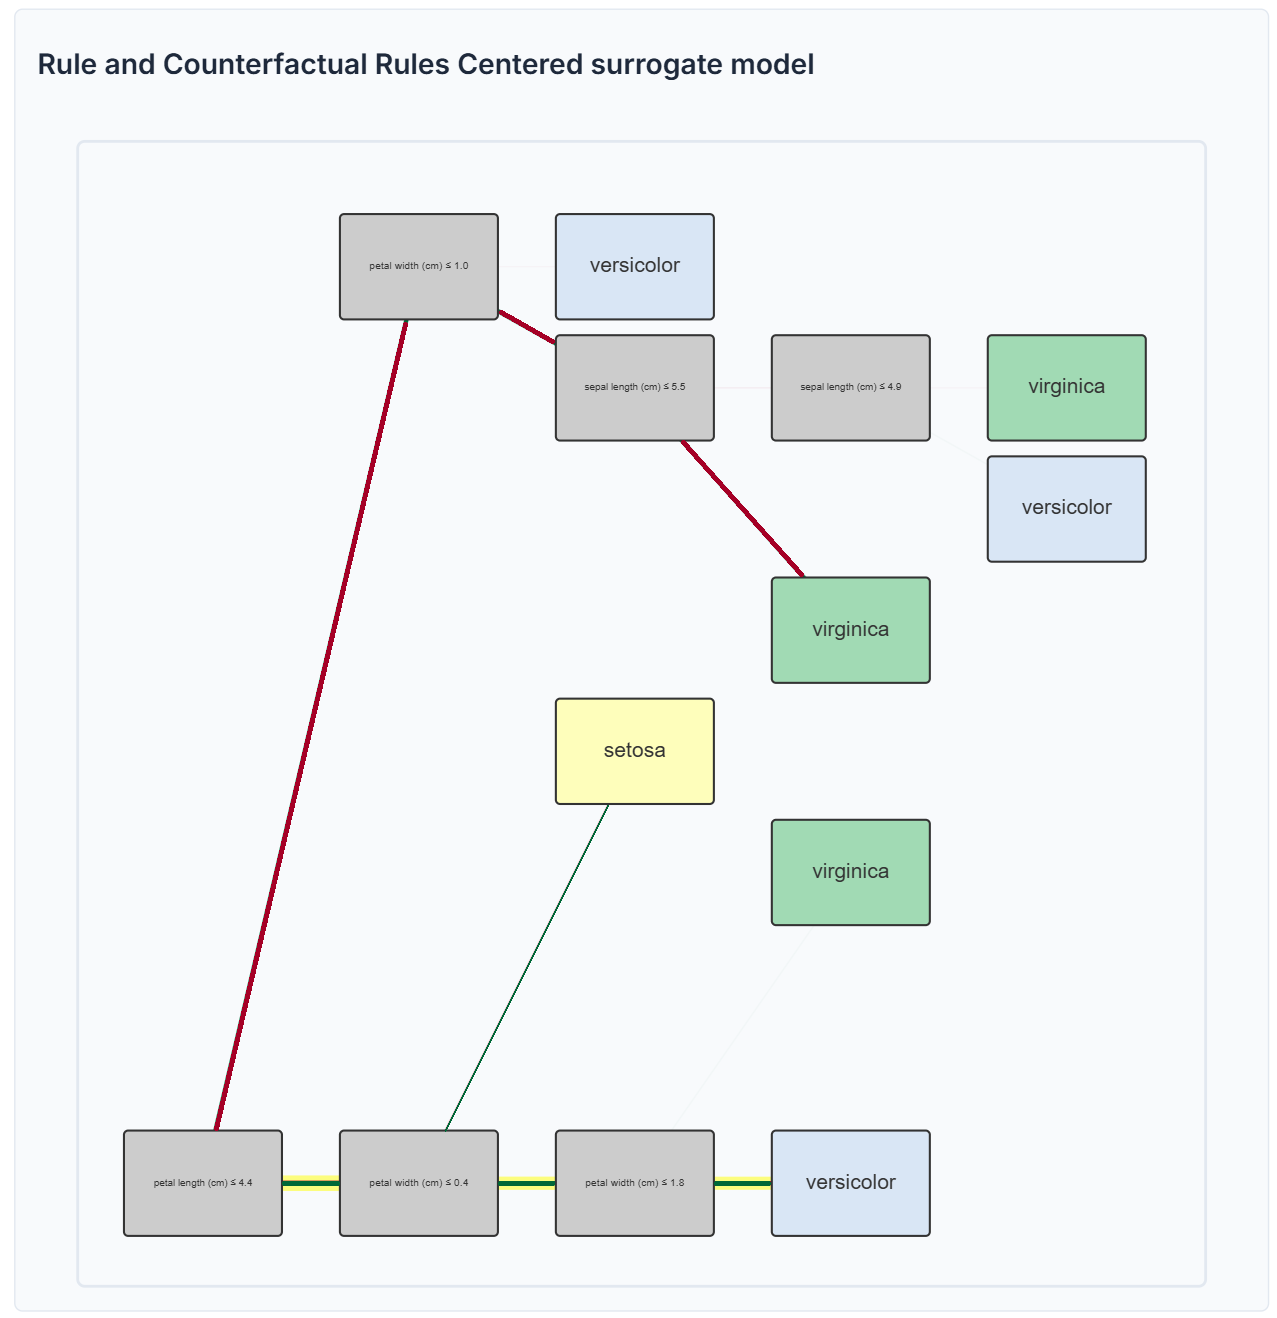
\includegraphics[width=\textwidth]{images/teaching_blocks_initial.png}
        \caption{Rule and Counterfactual Rules Centered surrogate model.}
        \label{fig:teaching_blocks_initial}
    \end{subfigure}
    \hfill
    % Two stacked images on the right
    \begin{subfigure}[c]{0.33\textwidth}
        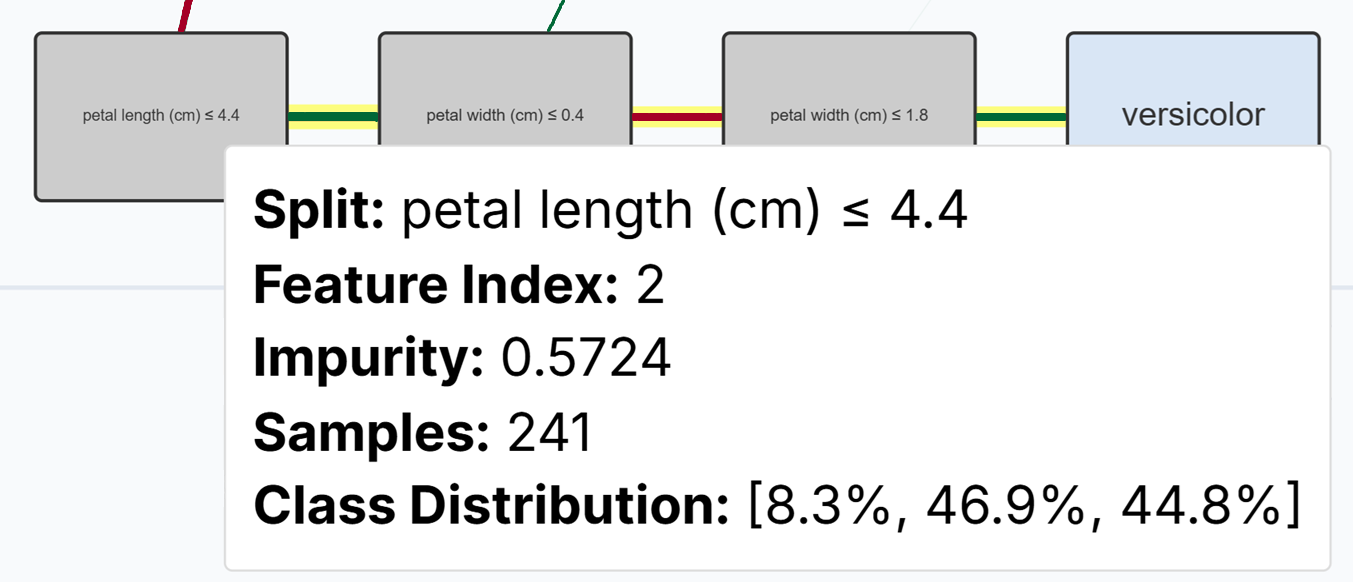
\includegraphics[width=\textwidth]{images/teaching_blocks_root_tooltip.png}
        \caption{Root node tooltip for the generated Rule and Counterfactual Rules Centered surrogate model.}
        \label{fig:teaching_blocks_root_tooltip}
        \vfill
        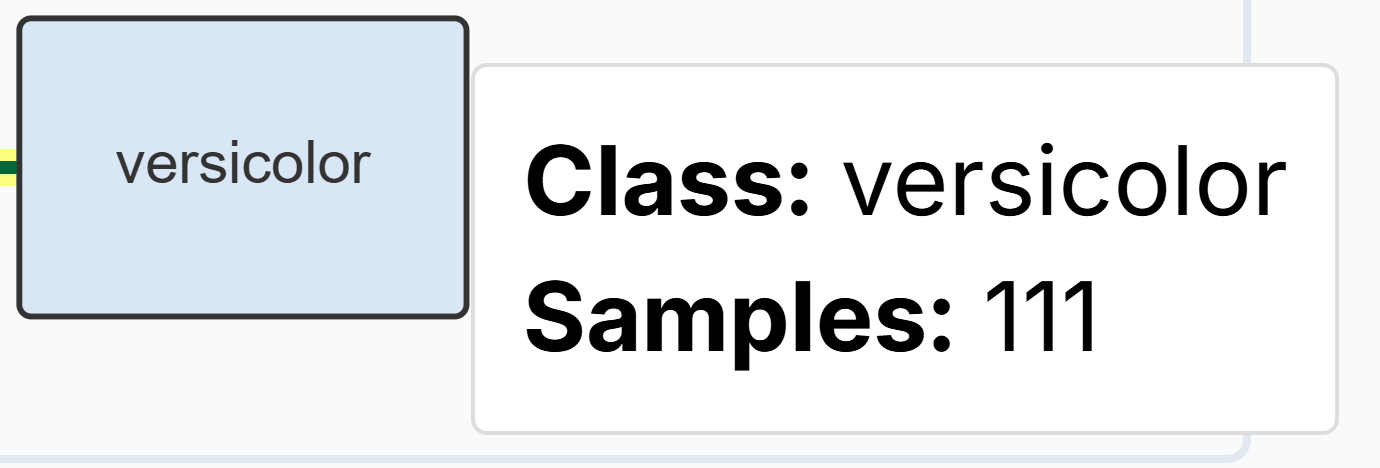
\includegraphics[width=\textwidth]{images/teaching_blocks_prediction_tooltip.png}
        \caption{Predicted class hover tooltip.}
        \label{fig:teaching_blocks_prediction_tooltip}
    \end{subfigure}
    \caption{Use case's Rule and Counterfactual Rules Centered surrogate model and details.}
\end{figure}

The teacher points to the virginica leaf nodes displayed throughout the tree above the highlighted path and talks about how the alternative paths represent counterfactual rules, otherwise said, different combinations of conditions that would lead to different predictions. For instance, if our flower had petal length less than 4.4 cm, petal width lower than 1 cm, sepal length lower than 5.5 it would have been classified as virginica regardless of other features. The rectangular nodes clearly display the predicted class in each leaf, with color-coding matching the scatter plot for visual consistency.

The teacher clicks on the Counterfactual alternative leaf node, as shown in Figure \ref{fig:teaching_blocks_click_alternative}. The system immediately highlights the corresponding points in the scatter plot above, mainly the cluster of green instances representing the virginica class at the bottom left of the scatter plot, and some points, originating from the dataset, near the decision boundary contested by virginica and versicolor instances. The teacher notes how this bidirectional coordination is crucial for building understanding, as they can see that these virginica instances occupy a specific region of the projected space, giving geometric intuition about the counterfactual scenario. 


\begin{figure}[ht]
    \centering
    \begin{subfigure}[c]{0.48\textwidth}
        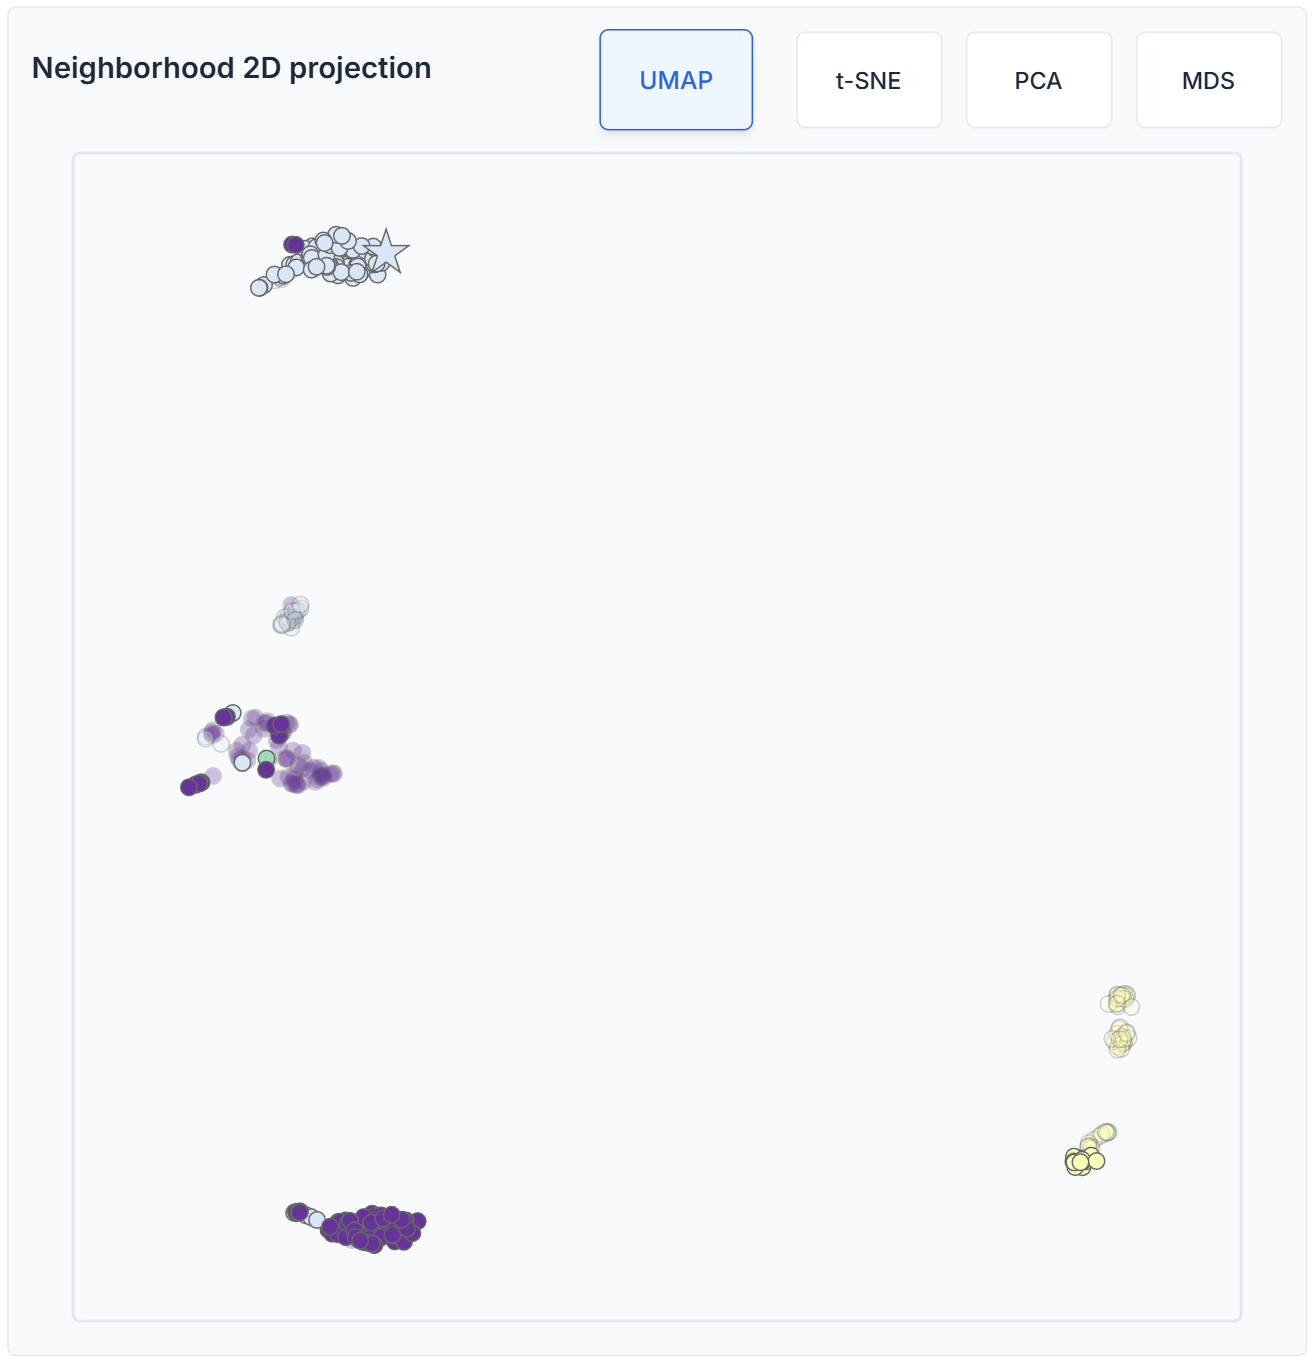
\includegraphics[width=\textwidth]{images/teaching_blocks_click_alternativeScatter.png}
        \caption{Neighborhood 2D projection.}
    \end{subfigure}
    \hfill
    \begin{subfigure}[c]{0.48\textwidth}
        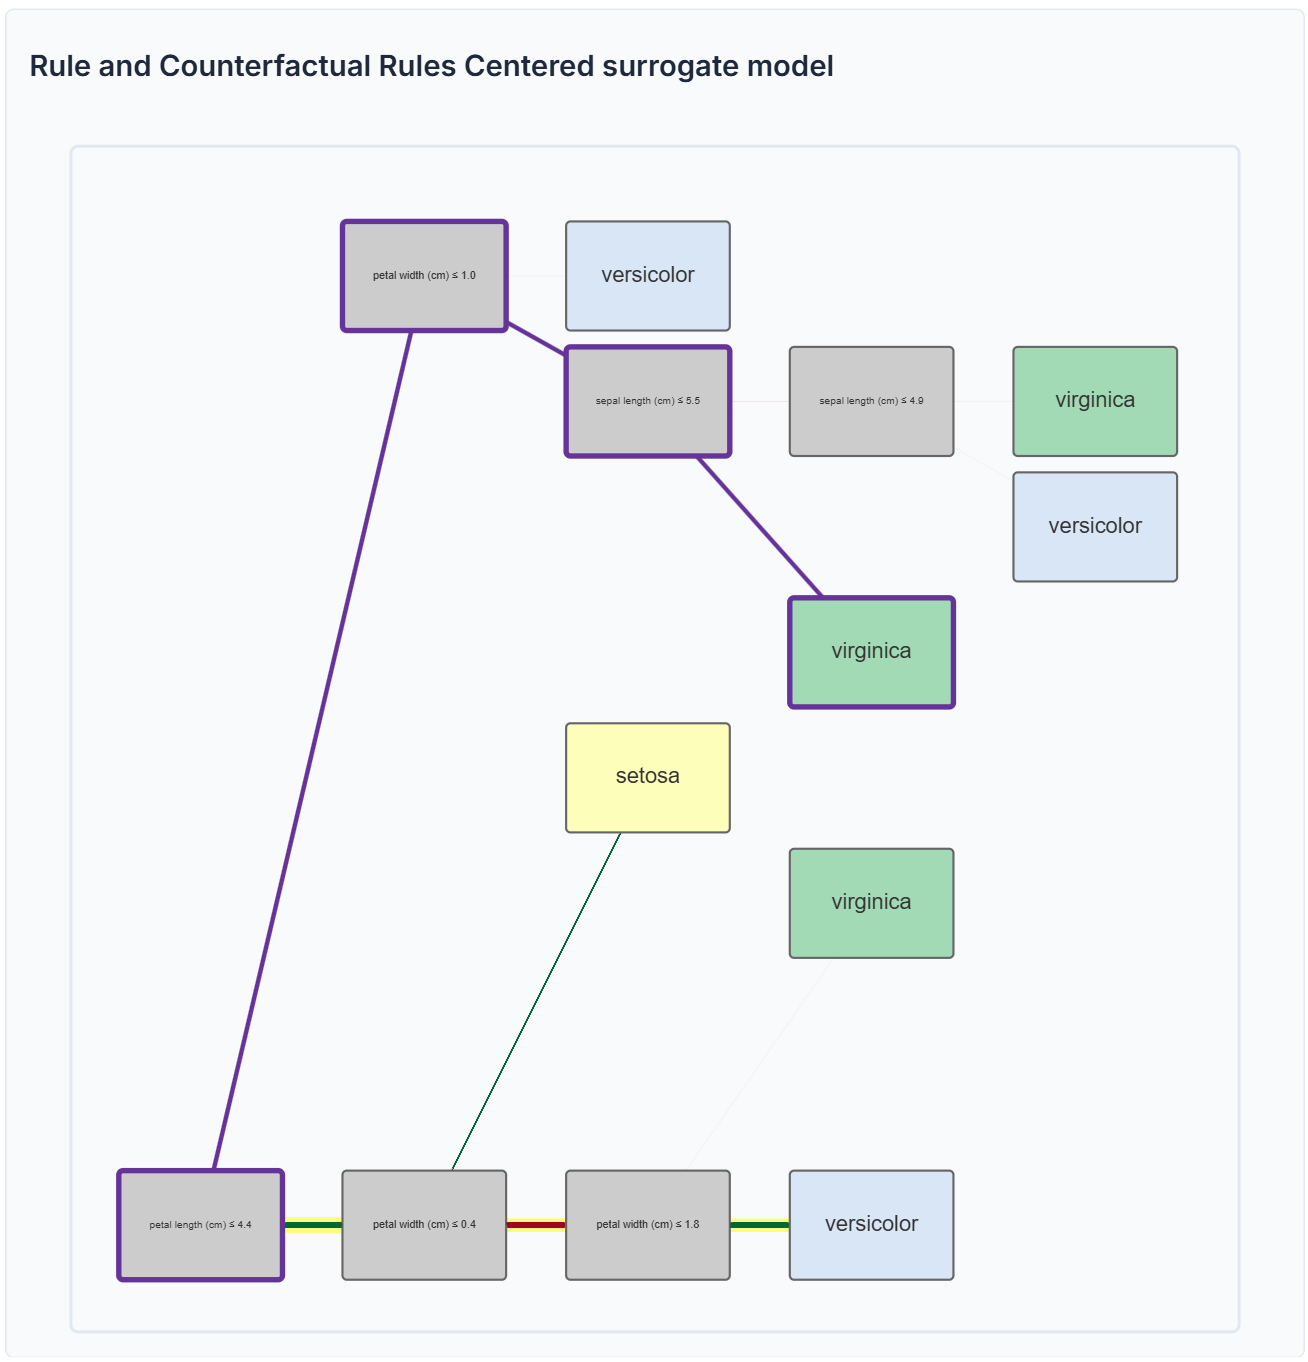
\includegraphics[width=\textwidth]{images/teaching_blocks_click_alternativeBlocks.png}
        \caption{Rule and Counterfactual Rules Centered surrogate model.}
    \end{subfigure}
    \caption{Click on counterfactual rule from the Rule and Counterfactual Rules Centered surrogate model visualization.}
    \label{fig:teaching_blocks_click_alternative}
\end{figure}


\subsection{Exploring Interaction Patterns and Coordination}

To deepen students' understanding of the coordination mechanism, the teacher demonstrates the reverse interaction flow. They click a purple point in the scatter plot's setosa cluster. The tree visualization immediately responds by highlighting the leftmost path from the root to the setosa leaf node. When any instance from the scatter plot is selected, the system automatically shows the decision path that the instance follows through the tree. This coordination helps in understanding the relationship between spatial position and logical conditions.

The teacher selects several points along the boundary between versicolor and virginica clusters, clicking each in succession. Students observe how the highlighted paths change, sometimes following similar routes but diverging at different split nodes. The teacher also highlights how instances near the decision boundary in the scatter plot correspond to paths that split at deeper levels in the tree. This showcases how the classifier needs more feature tests to distinguish between similar cases. The latter interactions are shown in Figure \ref{fig:teacherVariousInteractionsBlocks}.

The teacher hovers over a split node in the middle of the tree, and the tooltip reveals the number of samples that pass through the node and its value of impurity. The impurity measures shows how mixed the classes are at each decision point. High impurity means the genetic algorithm generated instances from multiple classes that satisfy the conditions leading to this node, which is exactly what is expected near decision boundaries. The teacher also points out how the traditional output included a fidelity score indicating how well the surrogate matches the black-box, but provided no insight into where and why the approximation might be imperfect. These per-node statistics give much finer-grained understanding of local explanation quality.

\begin{figure}[htbp]
    \centering

    % First pair
    \begin{subfigure}[c]{0.325\textwidth}
        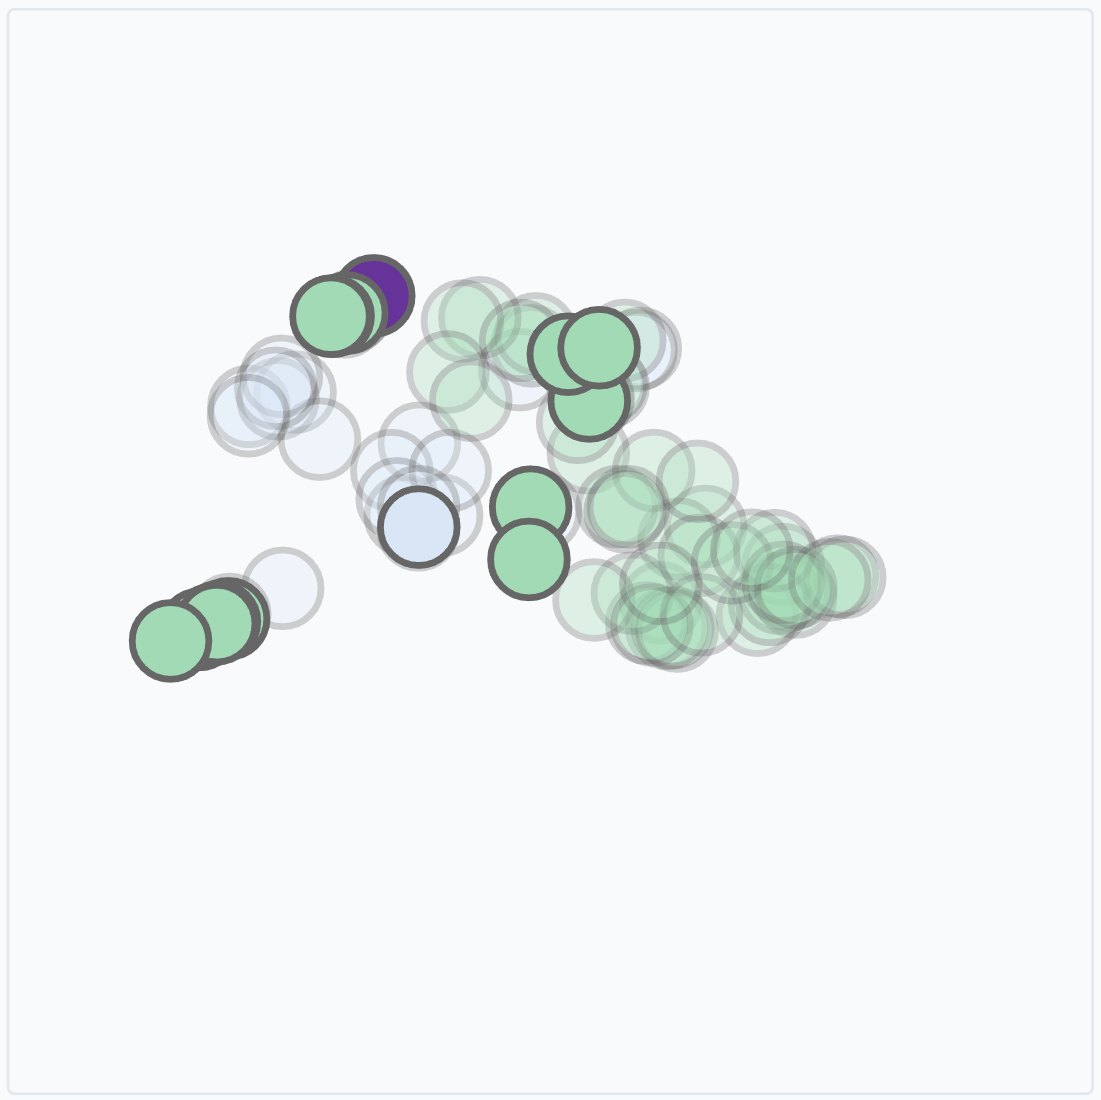
\includegraphics[width=\linewidth]{images/teacherVariousInteractionsBlocksScatter.png}
    \end{subfigure}
    \begin{subfigure}[c]{0.325\textwidth}
        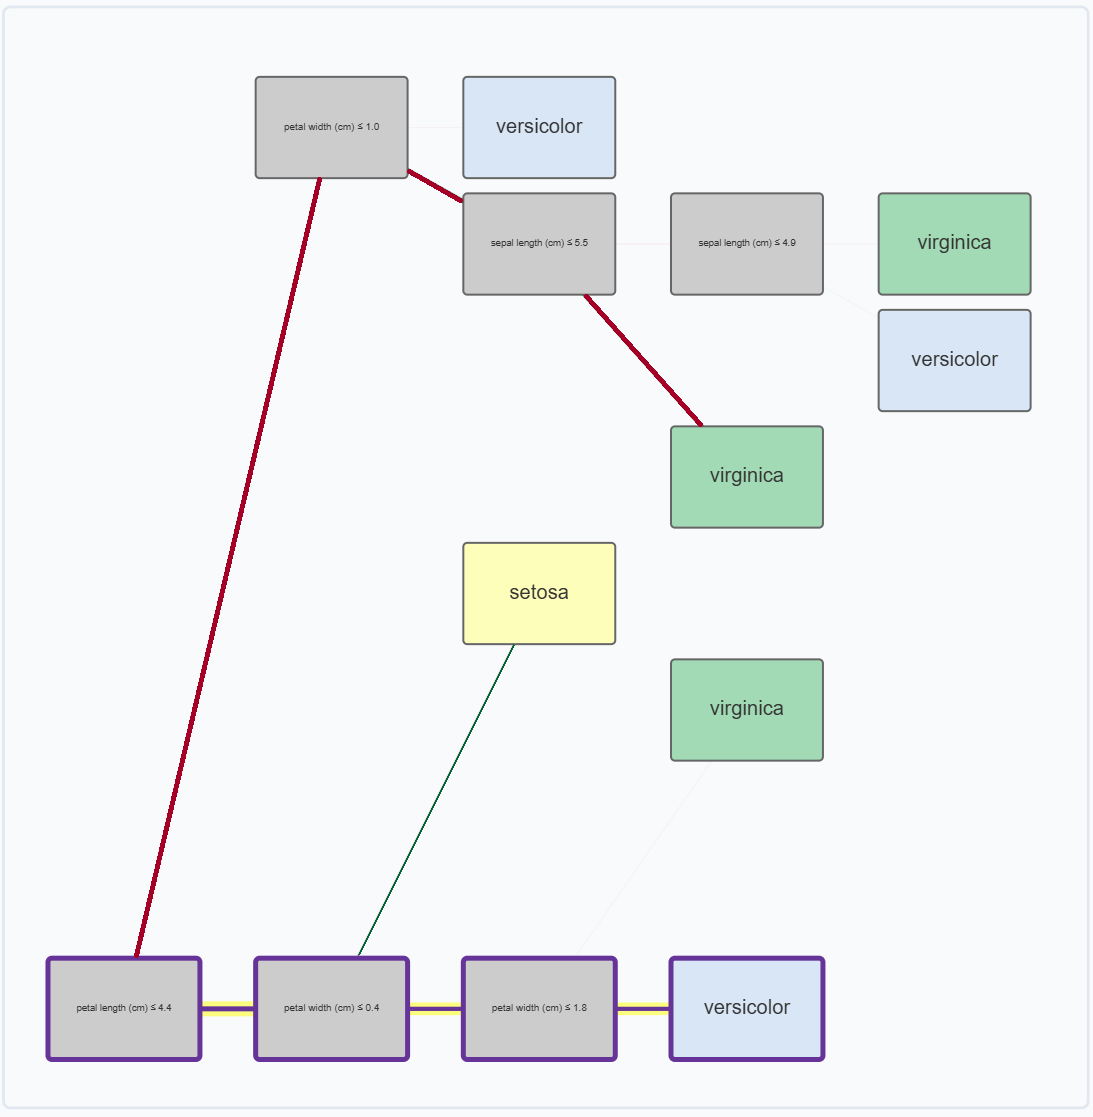
\includegraphics[width=\linewidth]{images/teacherVariousInteractionsBlocks.png}
    \end{subfigure}

    % Second pair
    \begin{subfigure}[c]{0.325\textwidth}
        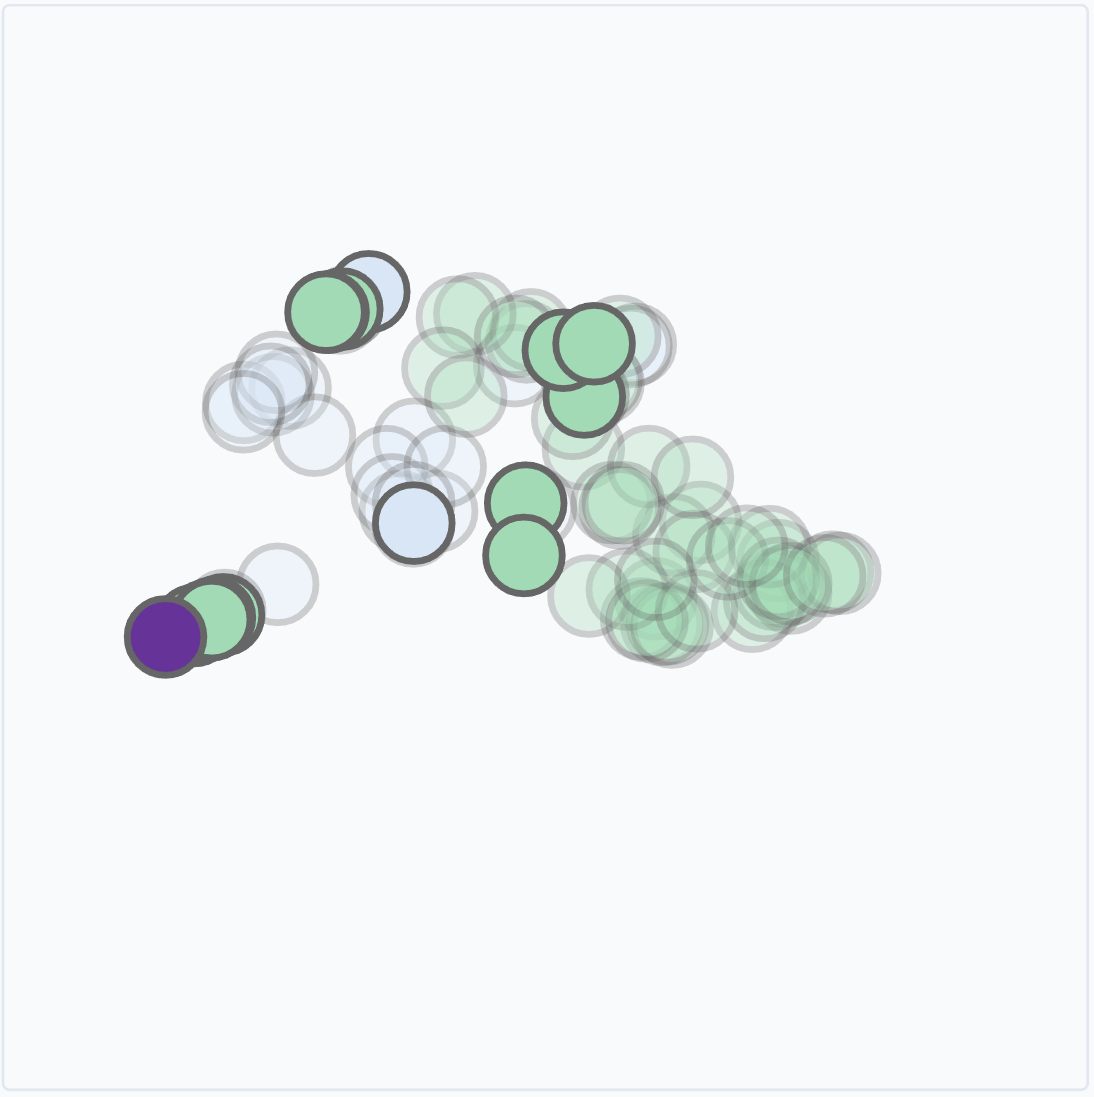
\includegraphics[width=\linewidth]{images/teacherVariousInteractionsBlocksScatter2.png}
    \end{subfigure}
    \begin{subfigure}[c]{0.325\textwidth}
        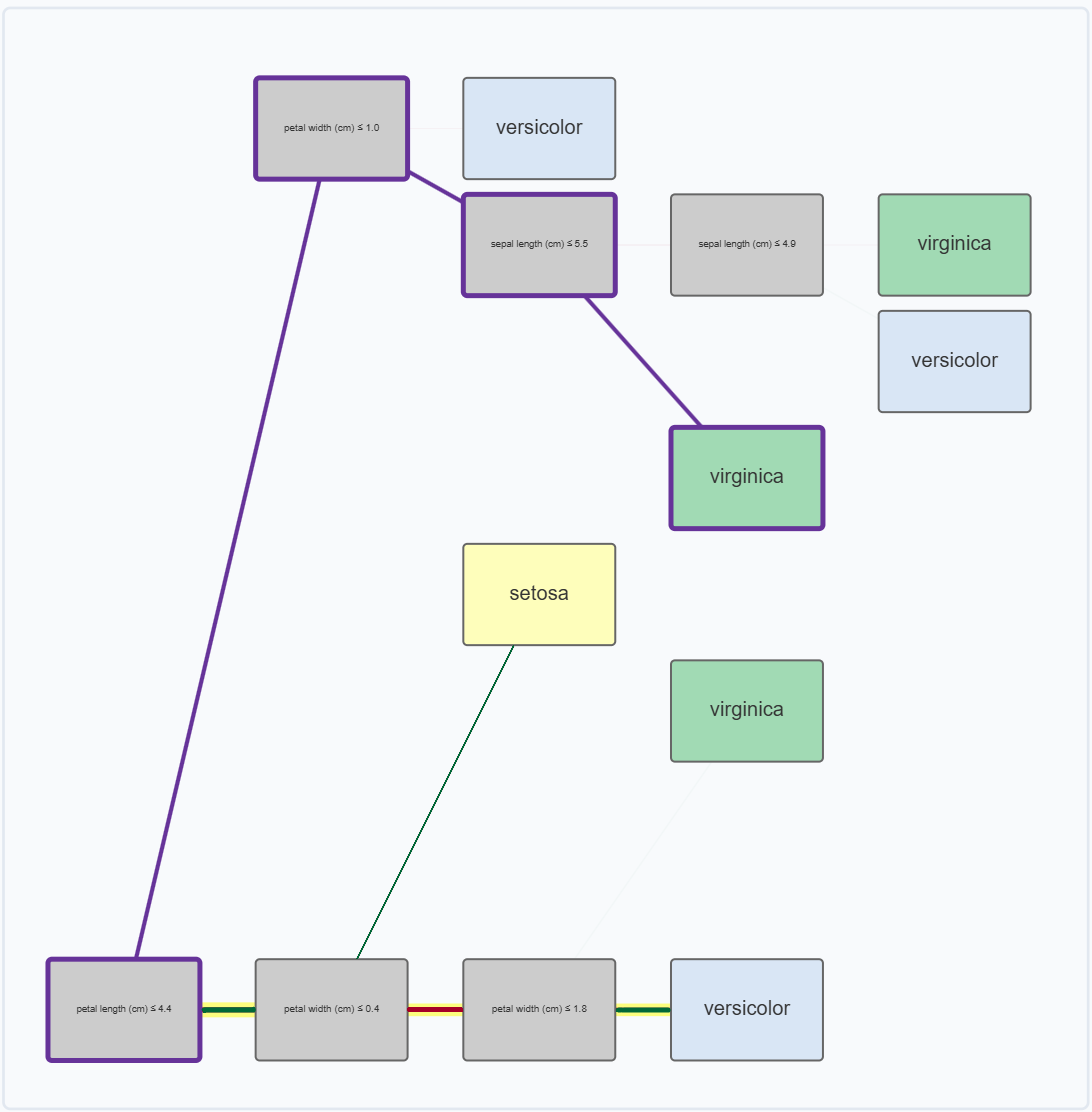
\includegraphics[width=\linewidth]{images/teacherVariousInteractionsBlocks2.png}
    \end{subfigure}

    % Third pair
    \begin{subfigure}[c]{0.325\textwidth}
        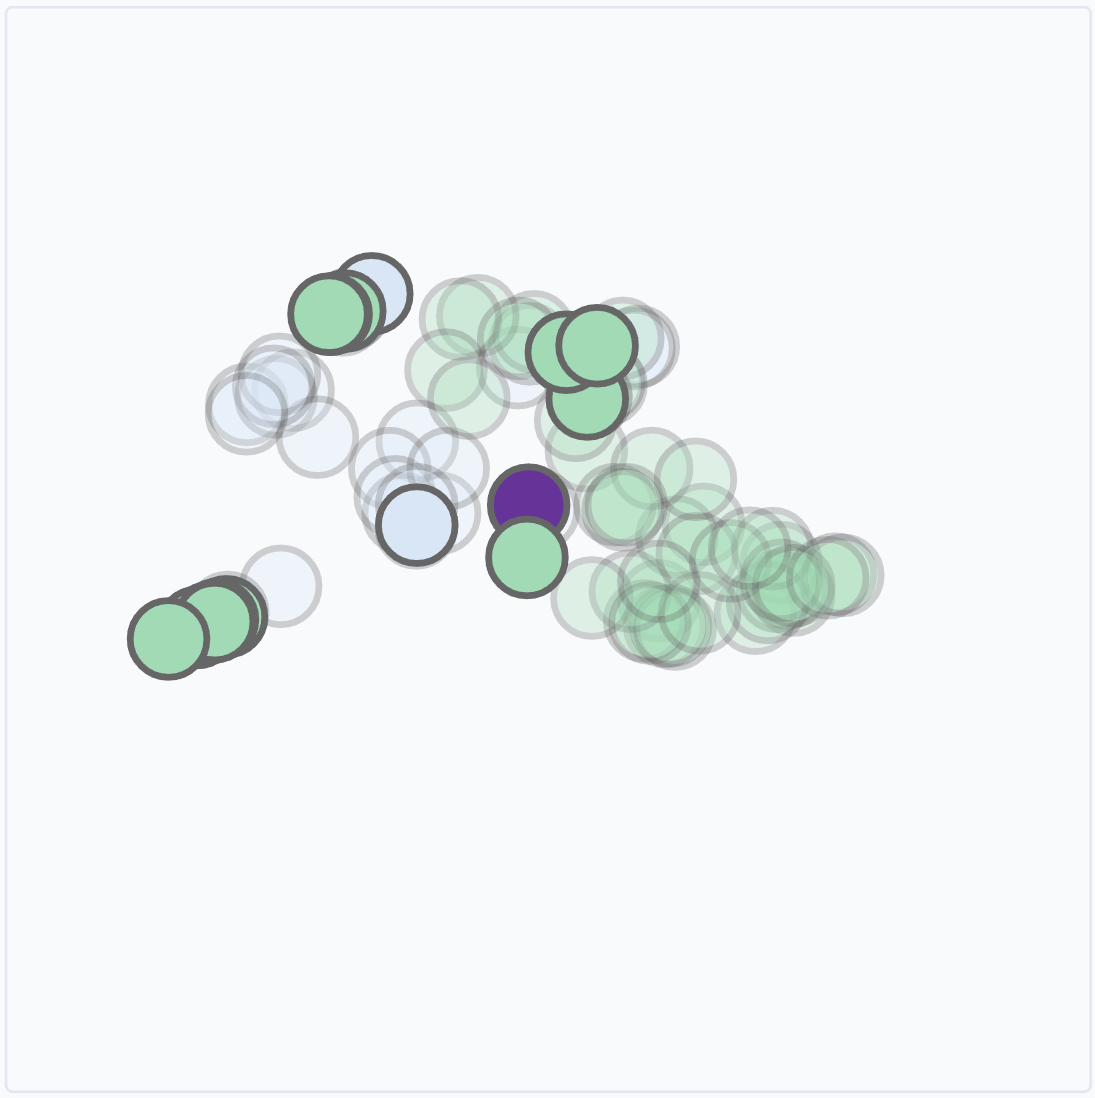
\includegraphics[width=\linewidth]{images/teacherVariousInteractionsBlocksScatter3.png}
    \end{subfigure}
    \begin{subfigure}[c]{0.325\textwidth}
        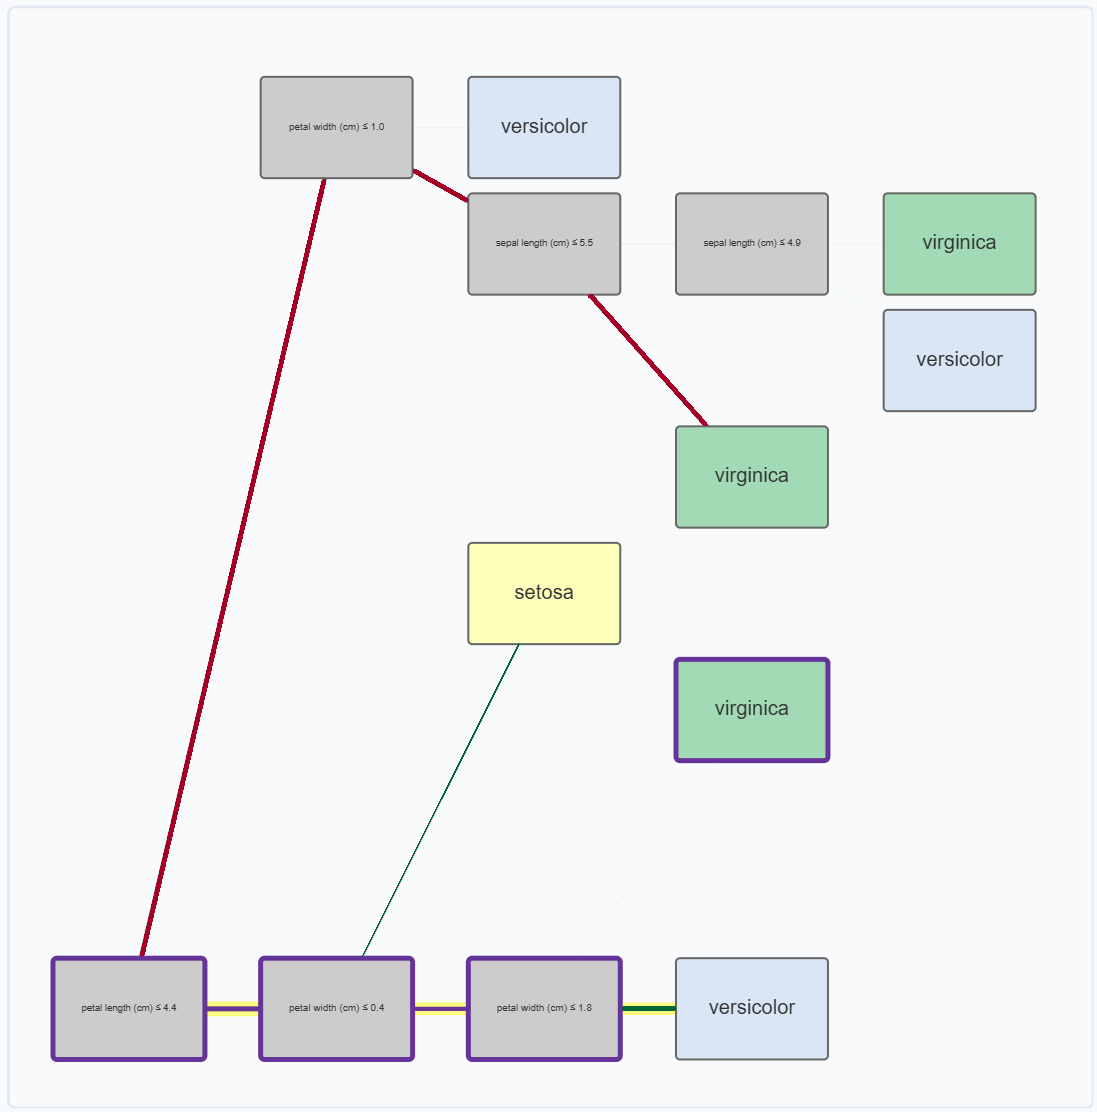
\includegraphics[width=\linewidth]{images/teacherVariousInteractionsBlocks3.png}
    \end{subfigure}

    % Fourth pair
    \begin{subfigure}[c]{0.325\textwidth}
        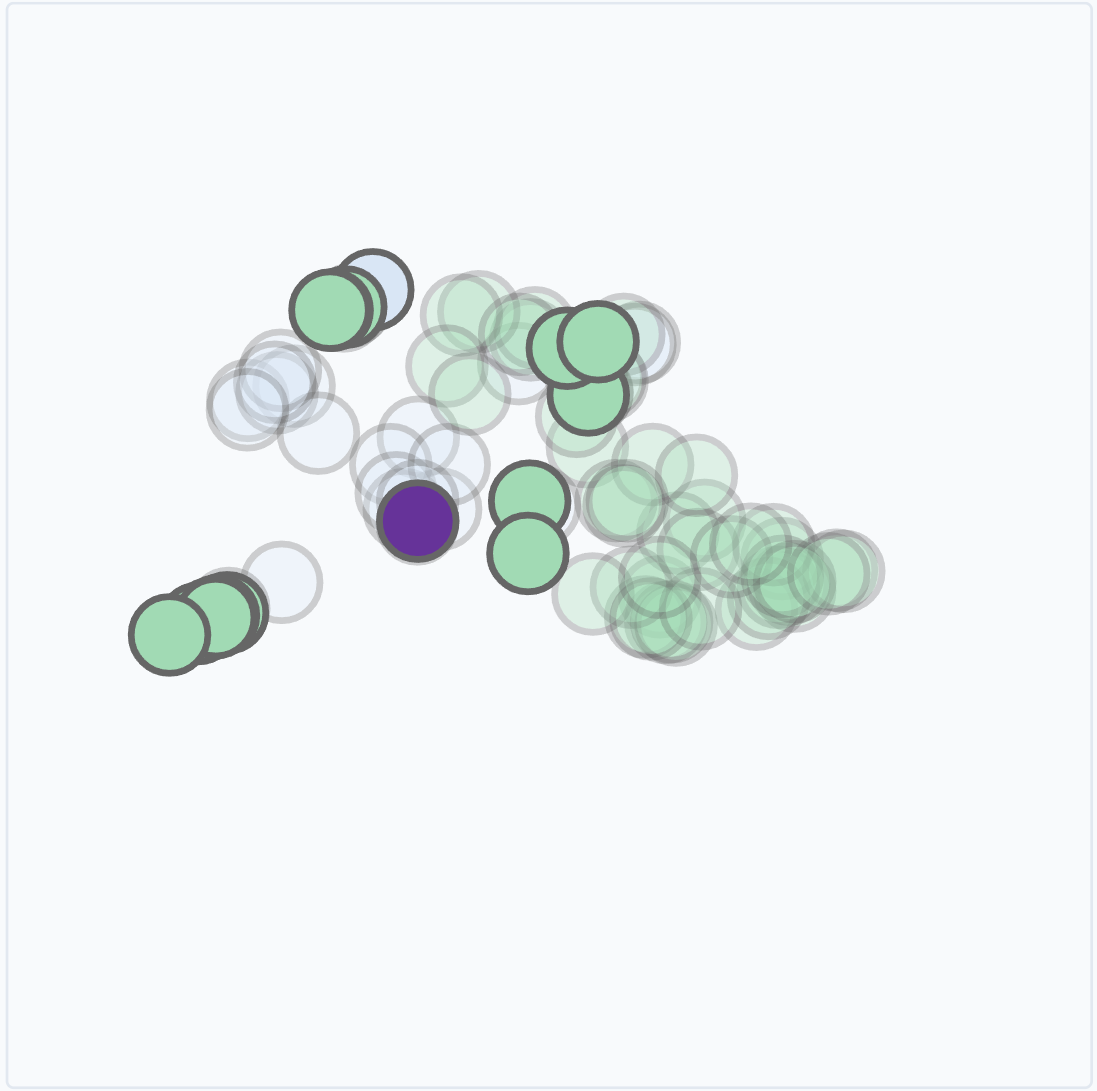
\includegraphics[width=\linewidth]{images/teacherVariousInteractionsBlocksScatter4.png}
    \end{subfigure}
    \begin{subfigure}[c]{0.325\textwidth}
        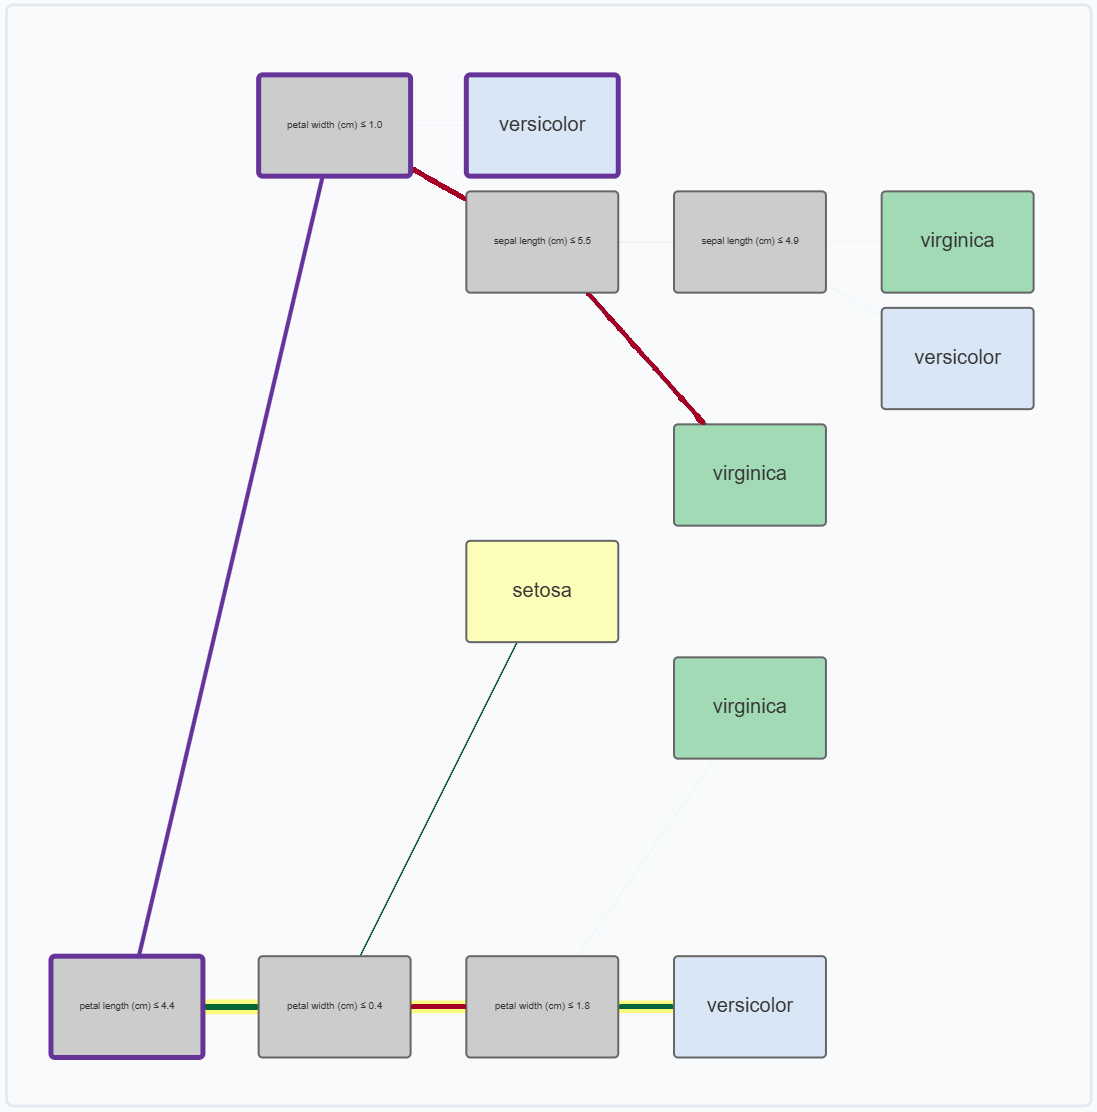
\includegraphics[width=\linewidth]{images/teacherVariousInteractionsBlocks4.png}
    \end{subfigure}

    \caption{Different interactions at the selection of points near the decision boundary.}
    \label{fig:teacherVariousInteractionsBlocks}
\end{figure}


\subsection{Comparing Tree Layout Alternatives}

Having established foundational understanding with the Rule and Counterfactual Rules Centered visualization, the teacher decides to demonstrate how different tree layouts can provide complementary insights. They change the visualization selection to Tree Layout, the visualization in Figure \ref{fig:teaching_classic_tree} appears.

The teacher explains that the traditional node-link tree layout uses circular nodes and emphasizes hierarchical relationships through vertical positioning. Students immediately notice the differences: nodes are positioned based on their depth and sibling relationships rather than aligned in horizontal rows, and the explained instance path uses only edge highlighting rather than also using the node positioning to draw attention.

The teacher clicks on a leaf node in the Tree Layout, observing the same bidirectional coordination with the scatter plot as the coordination mechanism remains consistent across different tree layouts. This consistency is important since the users of the interface can choose the layout that best fits the analytical goals without losing access to the same interaction capabilities.

Later, the teacher switches to the Rule Centered visualization, shown in Figure \ref{fig:teaching_spawn_tree}. Students notice immediately that only the explained instance path appears as rectangular nodes, while the alternative branches are represented as collapsed circular nodes with special markings to allow the maintenance of awareness of alternative scenarios. 

The teacher right-clicks on one of the collapsed subtree nodes, revealing a context menu with an \texttt{Expand Subtree} option. When they select it, the hidden branches unfurl, revealing the complete decision structure. The teacher explains how this progressive disclosure supports different depths of investigation. The teacher explains to the class that they can focus on the main explanation path and selectively explore alternatives only when needed, reducing visual complexity while maintaining access to complete information.

\begin{figure}[ht]
    \centering
    \begin{subfigure}[c]{0.48\textwidth}
        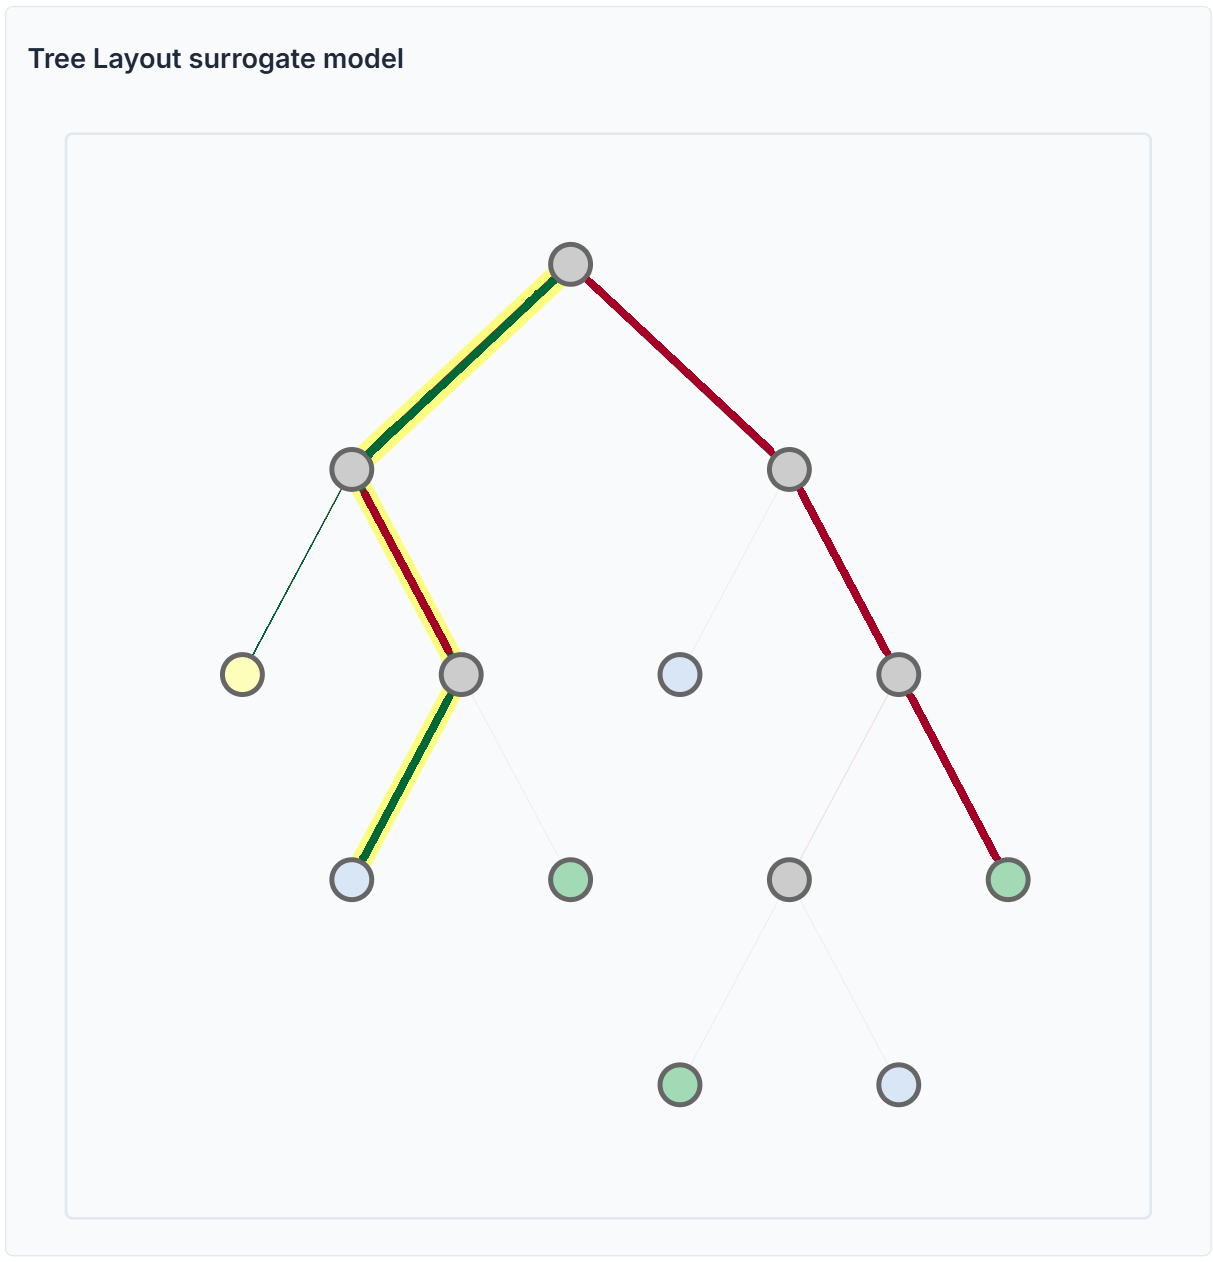
\includegraphics[width=\textwidth]{images/teaching_classic_tree.png}
        \caption{Tree layout surrogate model for the same tree previously analyzed by the teacher and class.}
        \label{fig:teaching_classic_tree}
    \end{subfigure}
    \hfill
    \begin{subfigure}[c]{0.48\textwidth}
        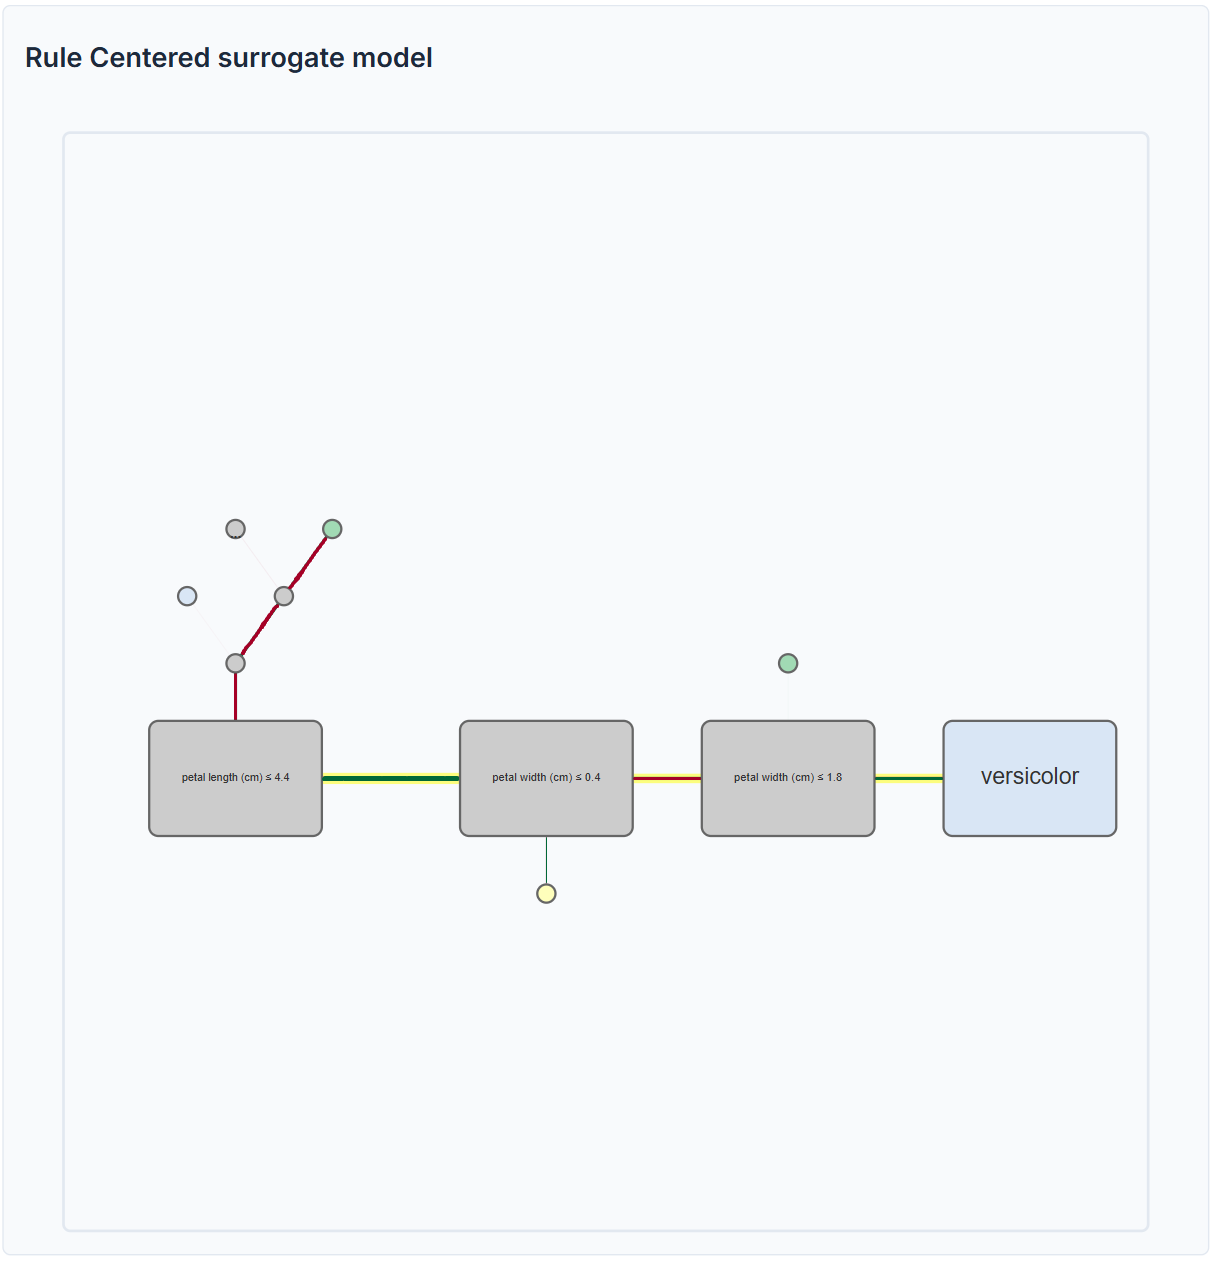
\includegraphics[width=\textwidth]{images/teaching_spawn_tree.png}
        \caption{Rule centered surrogate model visualization for the same tree previously analyzed by the teacher and class.}
        \label{fig:teaching_spawn_tree}
    \end{subfigure}
    \caption{Alternative visualizations shown in the teacher use case.}
\end{figure}

% \begin{figure}
%     \centering
%     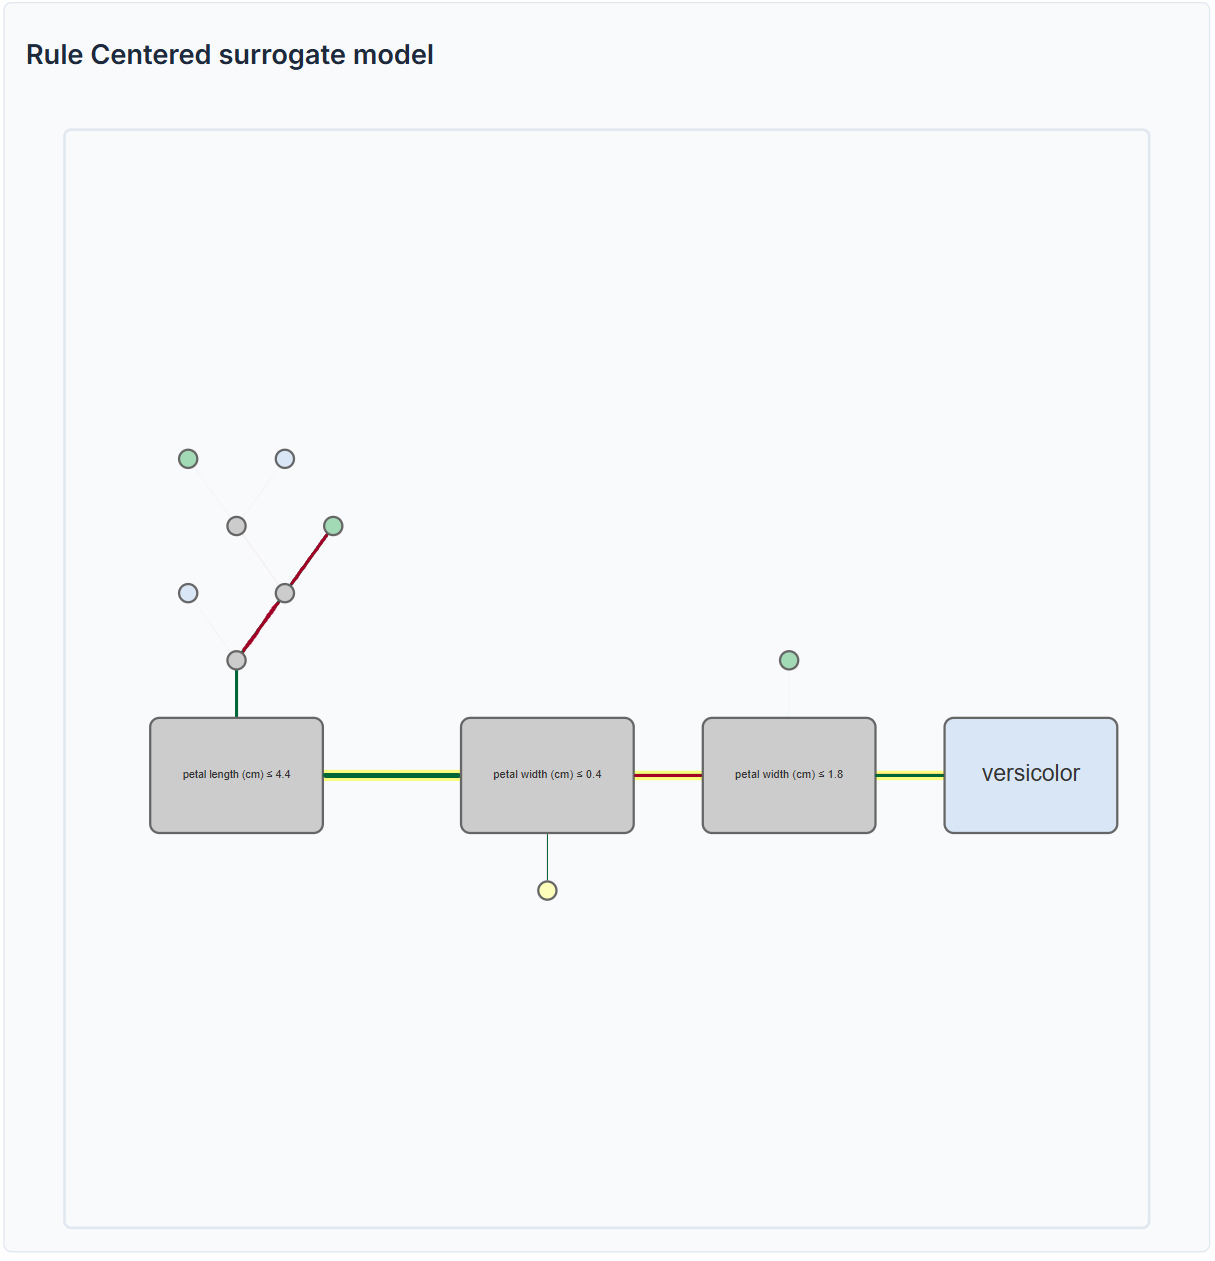
\includegraphics[width=0.5\linewidth]{images/teaching_spawn_tree_expanded.png}
%     \caption{Expanded version of the tree used}
%     \label{fig:placeholder}
% \end{figure}